
\chapter[Decomposition--Coordination methods by
  augmented...]{Decomposition--Coordination methods by augmented
  largrangian. Applications\protect
  \footnotemark[1]{}}\footnotetext[1]{This Chapter follows
  FORTIN-GLOWINSKI [1].}\label{chap5} 

\section{Introduction}\label{c5:s1}

\subsection{Motivation}\label{c5:ss1.1}
A large\pageoriginale number of problems in Mathematics, Physics, Mechanics, Economics,  etc... may be formulated as 
\begin{equation}
\min_{v \in V} \{F(Bv) + G(v) \} \tag{P}
\end{equation}
where 
\begin{enumerate}[-]
\item $V$, $H$ are topological vector spaces,
\item $B \in \mathscr{L}(V, H)$,
\item $F : H \to \overline{\mathbb{R}}$, $G : V \to
  \overline{\mathbb{R}}$ are convex, proper, l.s.c. functionals. 
\end{enumerate}
Let us give two examples taken from Chapter~\ref{chap2}.

\begin{example}\label{c5:exa1}%exa 1
It is the {\em Bingham flow problem} of Chapter~\ref{chap2}, 
Sec.~\ref{c2:s6}; we recall that $\Omega$ being a bounded domain of 
$\mathbb{R}^2$, we consider the variational problem   
\begin{equation}
\min_{v \in H^1_0(\Omega)} \{\frac{\nu}{2} \int_\Omega |\nabla v |^2 dx + g \int_\Omega  | \nabla v | dx - \int_\Omega fv dx\} \tag{1.1}\label{c5:eq1.1}
\end{equation}
where $\nu$ and $g$ are {\em positive} constants. Then \eqref{c5:eq1.1} is the particular problem $(P)$ in which
\begin{enumerate}[-]
\item  $V = H^1_0(\Omega)$,
\item  $H = L^2(\Omega) \times L^2(\Omega)$,
\item $B = \nabla$
\item $F(q) = \frac{\nu}{2} \int_\Omega |q|^2 dx + g \int_\Omega |q| dx, (|q| = \sqrt{q^2_1 + q^2_2}$,
\item $G(v) = - \int_\Omega fv dx$.
\end{enumerate}
Actually\pageoriginale  we can also take
\begin{enumerate}[-]
\item  $F(q) = g \int_\Omega |q|dx$,
\item $G(v) = \dfrac{\nu}{2}\int_\Omega  |\nabla v |^2 dx- \int _\Omega fv dx$.
\end{enumerate}
\end{example}

\begin{example}\label{c5:exa2}%example 2
It is {\em elastic-plastic torsion problem} of Chapter 2, Sec. 3; $\Omega$ being still bounded in $\mathbb{R}^2$, we consider 
\begin{equation}
\min_{v \in K}\{\frac{1}{2} \int_{\Omega}| \nabla v |^2 dx- \int_\Omega fv dx\} \tag{1.2}\label{c5:eq1.2}
\end{equation}
where 
$$
K = \{v \in H^1_0 (\Omega), | \nabla v | \leq 1 a.e.\}.
$$
\end{example}

Problem \eqref{c5:eq1.2} is the particular problem $(P)$ in which 
\begin{enumerate}[-]
\item $V = H^1_0(\Omega), H = L^2 (\Omega) \times L^2(\Omega)$,
\item $B = \nabla$,
\item $F(q)  = \dfrac{1}{2} \int_\Omega |q|^2 dx + I_{\hat{K}}(q)$,
\item $G(v)  = - \int_\Omega fv dx$,
\end{enumerate}
where $I_{\hat{K}}$ is the \textit{indicator functional} of the convex set 
$$
\hat{K} = \{ q \in H, |q| \leq 1 a.e.\},
$$
i.e.
\begin{equation*}
I_{\hat{K}}(q) =
\begin{cases}
0 \text{ if } q \in K\\
&\\
+\infty \text{ if }q \not \in K.
\end{cases}
\end{equation*}
We can also take
\begin{enumerate}[-]
\item $F (q)  = I_{\hat{K}}$,
\item $G(v)  = \dfrac{1}{2} \int_\Omega | \nabla v|^2 - \int_\Omega fv dx$.
\end{enumerate}
\textbf{Orientation.} Problems of type $(P)$ have a special structure and in the sequel we shall introduce iterative methods of solution taking it into account.

\subsection{Principle of the methods}\label{c5:ss1.2}% sub sec 1.2.

The\pageoriginale  decomposition-coordination methods to follow are
based on the following obvious \textit{equivalence} result: 

\begin{theorem}\label{c5:thm1.1}%theorem 1.1
$(P)$ {\em equivalent to}
\begin{equation}
 \min\limits_{\{v, q\} \in W } \{F (q) + G (v) \} \tag{$\Pi$}
\end{equation}
{\em where}
$$
W = \{\{ v, q\} \in V \times H, Bv-q = 0\}.
$$
\end{theorem}

\noindent
We shall assume in the sequel that $V$ and $H$ are \textit{Hilbert
  spaces} with inner products and norms respectively denoted by
$((\cdot,\cdot))$, $|| . ||$ and $(\cdot,\cdot)$ and $|.|$. We define then a
Lagrangian functional $\mathscr{L}$ associated to $(\pi)$, by  
\begin{equation}
\mathscr{L} (v, q, \mu) = F (q) + G (v) + (\mu, Bv-q), \tag{1.3}\label{c5:eq1.3}
\end{equation}
and for $r \geq 0$ an \textit{Augmented Lagrangian} $\mathscr{L}_r$ by 
\begin{equation}
\mathscr{L}_r (v, q, \mu) = \mathscr{L} (v, q, \mu) + \frac{r}{2} |Bv- q|^2.\tag{1.4}\label{c5:eq1.4}
\end{equation}

\begin{remark}\label{c5:rem1.1}%remark 1.1
Augmented Lagrangian methods for solving general optimization problems
have been introduced by HESTENES [\ref{k56:e1}], POWELL
[\ref{k78:e1}]. Augmented Lagrangian 
methods for solving problems like $(P)$ via $(\pi)$ have been
introduced by GLOWINSKI-MARROCCO [\ref{k54:e4}] and also
[\ref{k54:e5}]- [\ref{k54:e7}]. 
\end{remark}

\section[Properties of $(P)$ And of The Saddle-Points...]{Properties
  of $(P)$ And of The Saddle-Points of $\mathscr{L}$ And
  $\mathscr{L}_r$}\label{c5:s2}%sec 2. 

\subsection{Existence and uniqueness properties for 
(P).}\label{c5:ss2.1}% sub sec 2.1

Let define $J : V \to \overline{\mathbb{R}}$ by 
$$
J (v) = F (Bv) + G (v).
$$
Then $(P)$ can also be written 
\begin{equation}
\begin{cases}
J(u) \leq J (v) ~ \forall v \in V,\\
u \in V. \tag{2.1}\label{c5:eq2.1}
\end{cases}
\end{equation}
Let\pageoriginale  $j : X \to \overline{\mathbb{R}}$; we define the so-called \textit{domain} of $j(.)$ by 
$$
\text{ dom }(j) = \{x \in X, j(x) \in \mathbb{R}\}
$$
Then, if 
\begin{equation}
\text{ dom } (F \circ B) \cap \text{ dom } (G) \neq \phi, \tag{2.2}\label{c5:eq2.2}
\end{equation}
$J$ is \textit{convex, proper, l.s.c.} Therefore, \textit{sufficient}
conditions for $(P)$ to have a \textit{unique solution} are (cf. CEA
[\ref{k27:e1}], [\ref{k27:e2}], EKELAND-TEMAM [\ref{k43:e1}]): 
\begin{align*}
& - \lim\limits_{|| v || \to + \infty} F (v) = + \infty,\\
& - F \text{ strictly convex }.
\end{align*}

\begin{remark}\label{c5:rem2.1}%remark 2.1
If $B$ is an injection from $V$ to $H$, with $R(B)$ (= range of $B$) closed in $H$, then $|Bv|$ is a norm on $V$ equivalent  to $|| v ||$.
\end{remark}

\subsection{Properties of the saddle-points of $\mathscr{L}$ and 
$\mathscr{L}_r$}\label{c5:ss2.2}%sub sec 2.2

We have 

\begin{theorem}\label{c5:thm2.1}%theorem 2.1
Let $\{u, p, \lambda \}$ be a saddle-point of $\mathscr{L}$ on $V
\times H \times H$, then $\{u, p, \lambda \}$ is also a saddle-point
of $\mathscr{L}_r\, \forall r > 0$ and conversely. Moreover $u$ is
solution of $(P)$ and $p= Bu$. 
\end{theorem}

\begin{proof}
(i) Let $\{u, p, \lambda \}$ be a saddle-point of $\mathscr{L}$, then 
$\mathscr{L}(u, p, \lambda)  \in \mathbb{R}$ and 
\begin{equation}
\begin{cases}
\mathscr{L} (u, p, \mu) \leq \mathscr{L} (u, p, \lambda) \leq
\mathscr{L} (v, q, \lambda)  
\forall \{v, q, \mu \} \in V \times H \times H,\\
& \\
\{u, p, \lambda \} \in V \times H \times H.\tag{2.3}\label{c5:eq2.3}
\end{cases}
\end{equation}
\end{proof}
From the first inequality \eqref{c5:eq2.3} and from \eqref{c5:eq1.3}
it follows that  
$$
(\mu, Bu-p) \leq (\lambda, Bu-p)\, \forall _\mu \in H,
$$
which implies obviously that 
\begin{equation}
Bu = p. \tag{2.4}\label{c5:eq2.4}
\end{equation}\pageoriginale 
From the second inequality \eqref{c5:eq2.3} and from \eqref{c5:eq1.3}, \eqref{c5:eq2.4} it follows that 
\begin{equation}
J(u) = \mathscr{L} (u, p, \lambda) \leq (v, q, \lambda)\, \forall \{v, q \} \in V \times H\tag{2.5}\label{c5:eq2.5}
\end{equation}
Taking $q = Bv$ in \eqref{c5:eq2.5}, it follows from \eqref{c5:eq1.3} that 
\begin{equation}
J (u) \leq \mathscr{L} (v, Bv, \lambda) = J (v)\, \forall v \in V : \tag{2.6}\label{c5:eq2.6}
\end{equation}
hence $u$ is solution of $(P)$. Since $P = Bu$ we have 
\begin{equation}
\mathscr{L}_r (u, p, \mu) = \mathscr{L} (u, p, \mu) = J (u)\, \forall \mu \in H;  \tag{2.7}\label{c5:eq2.7}
\end{equation}
it follows then from \eqref{c5:eq2.3}, \eqref{c5:eq2.7} that 
\begin{equation}
\mathscr{L}_r (u, p, \mu) = \mathscr{L}_r (u, p, \lambda) \leq \mathscr{L} (v, q, \lambda)\, \forall \{v, q, \mu \} \in V \times H \times H. \tag{2.8}\label{c5:eq2.8}
\end{equation}
Since $\mathscr{L}_r (v, q, \mu)  = \mathscr{L} (v, q, \mu) + \dfrac{r}{2} |Bv-q|^2$, we obtain from \eqref{c5:eq2.8} that 
\begin{equation}
\mathscr{L}_r (u, p, \mu) \leq \mathscr{L}_r (u, p, \lambda) \leq \mathscr{L}_r (v, q, \lambda)\, \forall \{v, q, \mu \} \in V \times H \times H, \tag{2.9}\label{c5:eq2.9}
\end{equation}
which proves that $\{u, p, \lambda \}$ is also a saddle-point of $\mathscr{L}_r$ on $V \times H \times H$. To conclude this part of the proof we observe that from \eqref{c5:eq2.3}, $\{u, p \}$ is solution of 
\begin{equation}
\begin{cases}
\mathscr{L} (u, p, \lambda) \leq \mathscr{L}(v, q, \lambda)\, \forall \{v, q \} \in V \times H,\\
\{u, p\} \in V \times H, \tag{2.10}\label{c5:eq2.10}
\end{cases}
\end{equation}
from which it follows that $\{u, p \}$ is characterized (see CEA [1], [2], EKELAND - TEMAM [1])
\begin{equation}
\begin{cases}
F (q) - F (p) - (\lambda, q-p) \geq 0\, \forall q \in H,\\
p \in H, \tag{2.11}\label{c5:eq2.11}
\end{cases}
\end{equation}
\begin{equation}
\begin{cases}
G (v) - G (u) + (\lambda, B(v-u)) \geq 0\, \forall v \in V, \\
& \\
u \in V. \tag{2.12}\label{c5:eq2.12}
\end{cases}
\end{equation}\pageoriginale 
(ii) Let $\{u, p, \lambda \}$ be a saddle-point of $\mathscr{L}_r$ with $r > 0$. Then as in part (i) this implies that $p = Bu$ and that $u$ is  solution of $(P)$. Moreover, since $\{u, p, \lambda \}$ is solution of 
\begin{equation}
\begin{cases}
\mathscr{L}_r (u, p, \lambda) \leq \mathscr{L}_r (v, q, \lambda)\, \forall \{v, q \} \in V \times tH, \\
& \\
\{u, p \} \in V \times H,\tag{2.13}\label{c5:eq2.13}
\end{cases}
\end{equation}
it is characterized by 
\begin{equation}
\begin{cases}
F (q) - F (p)+ r (p-Bu, q-p)- (\lambda, q-p)\geq 0\, \forall q \in H, \\
& \\
p \in H,\tag{2.14}\label{c5:eq2.14} 
\end{cases}
\end{equation}
\begin{equation}
\begin{cases}
G (v) - G(u) + r (Bu-p, B (v-u)) + (\lambda, B(v-u)) \geq 0\, \forall v  \in V, \\
& \\
u \in V. \tag{2.15}\label{c5:eq2.15}
\end{cases}
\end{equation}
But since $Bu - p = C$,  \eqref{c5:eq2.14}, \eqref{c5:eq2.15} reduce
to \eqref{c5:eq2.11}, \eqref{c5:eq2.12} and this fact implies that
$\{u, p, \lambda \}$ satisfies \eqref{c5:eq2.10}. It follows then from
\eqref{c5:eq2.7} that $\{u, p, \lambda \}$ satisfies \eqref{c5:eq2.3}
and this completes the proof of the theorem. 

\section{Description of The Algorithms}\label{c5:s3}%sec 3

It follows from Theorem \ref{c2:thm2.1} that a way of solving $(P)$ is to solve
the saddle point problem  
\begin{equation}
\begin{cases}
\mathscr{L}_r (u, p, \mu) \leq \mathscr{L}_r (u, p, \lambda) \leq (v,
q, \lambda)\, \forall \{v, q, \mu \} \in V \times H \times H, \\
& \\
\{u, p, \lambda \} \in V \times H \times H. \tag{3.1}\label{c5:eq3.1}
\end{cases}
\end{equation}
To do so we shall (See CEA [1], G.L.T [1, Ch. 2]) and algorithm of Uzawa's type and a variant of it.

\subsection{First algorithm}\label{c5:ss3.1}%sub sec 3.1

We denote\pageoriginale  by ALG 1 the following algorithm:
\begin{equation}
\lambda^0 \in H \text{ given }, \tag{3.2}\label{c5:eq3.2}
\end{equation}
\textit{then} $\lambda^n$ \textit{known, we define} $u^n$, $p^n$, $\lambda^{n+1}$ \textit{by}
\begin{equation}
\begin{cases}
\mathscr{L}_r (u^n, p^n, \lambda^n) \leq \mathscr{L}_r (v, q, \lambda^n) 
\forall \{v, q \} \in V \times H, \\
& \\
\{u^n, p^n \} \in V \times H, \tag{3.3}\label{c5:eq3.3}
\end{cases}
\end{equation}
\begin{equation}
\lambda^{n+1} = \lambda^{n} + \rho_n (Bu^n - p^n), \rho_n > 0.\tag{3.4}\label{c5:eq3.4}
\end{equation}
The problem \eqref{c5:eq3.3} is in fact equivalent to the following system of 
\textit{two coupled variational inequalities} (of the second kind):
\begin{equation}
\begin{cases}
G (v) - G (u^n) + (\lambda^n, B(v-u^n))+ r (Bu^n - p^n, B (v-u^n))
\geq 0\, \forall v  \in V, \\ 
& \\
u^n \in V, \tag{3.5}\label{c5:eq3.5}
\end{cases}
\end{equation}
\begin{equation}
\begin{cases}
F (q) - F (p^n) - (\lambda^n, q-p^n) + r (p^n - Bu^n, q-p^n) \geq 0\, \forall q \in H,\\
& \\
p^n \in H.\tag{3.6}\label{c5:eq3.6}
\end{cases}
\end{equation}
The convergence of ALG 1 will be studied in Sec. \ref{c5:s4}.
  
\subsection{Second algorithm}\label{c5:ss3.2}% sub sec 3.2.
  
The main drawback of ALG 1 is that it requires at each interaction the solution of the coupled EVIs \eqref{c5:eq3.5}, \eqref{c5:eq3.6}. To overcome thus difficulty it is natural to consider the following variant of ALG 1 (denoted ALG 2  in the following):
  \begin{equation}
\{p^0 , \lambda ^1 \} \in H \times H \text{ given }, \tag{3.7}\label{c5:eq3.7}
 \end{equation}  
\textit{then} $\{ p^{n-1}, \lambda^n \}$ \textit{known, we define} $\{ u^n, p^n, \lambda^{n+1} \}$ \textit{by}
{\fontsize{10}{12}\selectfont
\begin{equation}
\begin{cases}
G (v) - G (u^n) + (\lambda^n, B (v-u^n))  + r (Bu^n - p^{n-1}, B (v-u^n)) \geq 0\, \forall v \in V, \\
& \\
u^n \in V, \tag{3.8}\label{c5:eq3.8}
\end{cases}
\end{equation}}\relax
\begin{equation}
\begin{cases}
F(q) - F (p^n) - (\lambda^n, q-p^n) + r (p^n - Bu^n, q-p^n) \geq 0\, \forall q \in H, \\
& \\
p^n \in H, \tag{3.9}\label{c5:eq3.9}
\end{cases}
\end{equation}\pageoriginale 
\begin{equation}
\lambda^{n+1} = \lambda^n \rho_n (Bu^n - p^n), \rho_n > 0. \tag{3.10}\label{c5:eq3.10}
 \end{equation}
 The convergence  of ALG 2 will be studied in Sec. 5.
 
\section{Convergence of Alg 1}\label{c5:s4}% sec 4
 
\subsection{General case}\label{c5:ss4.1}% subsec 4.1
 
 In this subsection $V$ and $H$ are possibly \textit{infinite dimensional}; we assume that of course
 \begin{equation}
\text{ dom } (F \circ B) \cap \text{ dom } (G) \neq \phi, \tag{4.1}\label{c5:eq4.1}
 \end{equation} 
 and also 
 \begin{equation}
B \text{ is an injection and } R (B) \text{ is closed in }H.\tag{4.2}\label{c5:eq4.2}
\end{equation} 
We assume also that 
\begin{equation}
\lim\limits_{|q| \to + \infty} \frac{F (q)} {|q|} = + \infty, \tag{4.3}\label{c5:eq4.3}
\end{equation}  
\begin{equation}
F = F_0 + F_1 \text{ with } F_0, F_1 \text{ convex , proper, l.s.c. }, 
\end{equation} 
\begin{equation}
\begin{cases}
F_0 \text{ is Gateaux-differentiable and uniformly convex on the }\\
& \\
\text{ bounded sets of }H.\tag{4.5}\label{c5:eq4.5}
\end{cases}
\end{equation}
By definition we say that $F_0$ is \textit{uniformly convex} on the
bounded sets of $H$ if the following property holds: 
\begin{equation}
\begin{cases}
\forall M > 0, \exists ~\delta_M : [0, 2M] \to \mathbb{R},
\text{continuous, strictly increasing with }\\ 
\delta_M (0) = 0,  \text{ such that }\, \forall q, p \in H \text{ with } |p|  \leq M, |q| \leq M \text{ we have }\\
(F'_0 (q) - F'_0, q-p) \geq \delta_M (|q-p|), \tag{4.6}\label{c5:eq4.6}
\end{cases}
\end{equation} 
where $F'_0 \bigtriangledown F_0$ is the $G$-derivative of $F_0$. From the above properties, $(P)$ has a \textit{unique solution} $u$ and we define $p \in H$ by $p = Bu$.
 
\begin{exercise}\label{c5:exer4.1}%exercise 4.1
Prove\pageoriginale  that $(P)$ is well-posed if \eqref{c5:eq4.1}--\eqref{c5:eq4.5} hold.
\end{exercise}  
 About the convergence of ALG 1 we have 
\begin{theorem}\label{c5:thm4.1}%theorem 4.1
We assume that $\mathscr{L}$ has a saddle-point $\{u, p, \lambda \}  \in V \times H \times H$. Then under the above assumption on $B$, $F$, $G$ and if 
\begin{equation}
0 < \alpha_0 \leq \rho_n \leq \alpha_1 < 2r \tag{4.7}\label{c5:eq4.7}
 \end{equation} 
 the following convergence properties hold 
 \begin{align*}
& u^n  \to u \text{ strongly in } V,  \tag{4.8}\label{c5:eq4.8}\\
& P^n \to P = Bu \text{ strongly in } H, \tag{4.9}\label{c5:eq4.9}\\
& \lambda^{n+1} - \lambda^n \to 0 \text{ strongly in } H,
   \tag{4.10}\label{c5:eq4.10}\\ 
& \lambda^n \text{ is  bounded in }H. \tag{4.11}\label{c5:eq4.11}
 \end{align*}
 Moreover if $\lambda^*$ is weak cluster point of $\{\lambda^n \}_n$ in $H$, then $\{u, p, \lambda^* \}$ is a saddle-point of $\mathscr{L}_r$ over $V \times H \times H$.
\end{theorem}  
  
\begin{proof}
Since $\{u, p, \lambda \}$ is a saddle-point of $\mathscr{L}_r$ we have
\begin{equation}
\begin{cases}
\mathscr{L}_r (u, p, \lambda) \leq \mathscr{L}_r (v, q, \lambda)\, \forall \{v, q \} \in V \times H, \\
& \\
\{u, p \} \in V \times H. \tag{4.12}\label{c5:eq4.12}
\end{cases}
\end{equation}
Therefore $\{u, p \}$ is characterized by 
\begin{equation}
\begin{cases}
G (v) - G (u) + (\lambda, B (v-u)) + r (Bu - q, B (v-u))\\ 
\hspace{6.5cm} \geq 0\, \forall v \in V, \\ 
u \in V,\tag{4.13}\label{c5:eq4.13}
\end{cases}
\end{equation}
\begin{equation}
\begin{cases}
(F'_0 (p), q-p) + F_1 (q) - F _1 (p) - (\lambda, q-p)\\ 
  \hspace{4cm} + r (p - Bu,  q-p) \geq 0\, \forall q \in H, \\ 
p \in H. \tag{4.14}\label{c5:eq4.14}
\end{cases}
\end{equation}
Moreover we have, from Theorem~\ref{c5:thm2.1}, $Bu = p$; therefore 
\begin{equation}
\lambda = \lambda + \rho_n (Bu - p).\tag{4.15}\label{c5:eq4.15}
\end{equation}
    Let\pageoriginale  us define $u^{-n}$, $p^{-n}$, $\lambda^{-n}$ by 
  $$
  u^{-n} = u^n -u, p^{-n} = p^n - p, \lambda^{-n} = \lambda^n - \lambda.
  $$
  It follows then from \eqref{c5:eq3.4}, \eqref{c5:eq4.15} that 
  $$
  \lambda^{-n+1} = \lambda^{-n} + \rho_n (Bu^{-n} - p^{-n}).
  $$
  which implies 
  $$
|\lambda^{-n+1}|^2 = |\lambda^{-n}|^2 + 2\rho_n (\lambda^{-n}, Bu^{-n} 
- p^{-n}) + \rho_n^2 |B u^{-n} - p^{-n}|^2
  $$
  or, what will be more convenient, 
  \begin{equation}
 |\lambda^{-n+1}|^2 = |\lambda^{-n}|^2 + 2\rho_n (\lambda^{-n}, Bu^{-n} - p^{-n}) + \rho_n^2 |B u^{-n} - p^{-n}|^2.\tag{4.16}\label{c5:eq4.16}
\end{equation}
since $\{u^n, p^n \}$ is solution of \eqref{c5:eq3.3} it is characterized by 
\begin{equation}
\begin{cases}
G (v) - G (u^n) + (\lambda^n, B (v-u^n) ) + r (Bu^n - p^n, B(v-u^n)) \geq 0\, \forall v \in V,\\
& \\
u^n \in V, \tag{4.17}\label{c5:eq4.17}
\end{cases}
\end{equation}
\begin{equation}
\begin{cases}
(F'_0 (p^n), q-p^n) + F_1 (q) - F_1 (p^n) - (\lambda^n, q-p^n)\\ 
  \hspace{3cm}+ r (p^n - Bu^n, q-p^n) \geq 0\, \forall q \in H,\\
  p^n \in H.\tag{4.18}\label{c5:eq4.18}
\end{cases}
\end{equation}  
Taking $v = u$ (\resp. $v = u^n$) in \eqref{c5:eq4.17}
(\resp. \eqref{c5:eq4.13}) and $q = p$ (\resp. $q = p^n$) in
\eqref{c5:eq4.18} (\resp . \eqref{c5:eq4.14}) we obtain by addition 
\begin{equation}
(\lambda^{-n}, Bu^{-n}) + r (Bu^{-n} - p^{-n}, B u^{-n}) \leq 0,
  \tag{4.19}\label{c5:eq4.19} 
\end{equation}
\begin{equation}
(F'_0 (p^n) - F'_0 (p), p^{-n})- (\lambda^{-n}, p^{-n}) + r (p^{-n} -
  Bu^{-n}, p^{-n}) \leq 0, \tag{4.20}\label{c5:eq4.20} 
\end{equation}
which imply, also by addition,
$$
(\lambda^{-n}, Bu^{-n} -  p^{-n}) + (F'_0 (p^n) -  F'_0 (p), p^{-n}) +
r |Bu^{-n} - p^{-n}|^2 \leq 0,  
$$
i.e.
\begin{equation}
- (\lambda^{-n}, B u^{-n} - p^{-n}) \geq (F'_0 (p^n) - F'_0 (p), p^{-n}) + r |Bu^{-n} - p^{-n}|^2.\tag{4.21}\label{c5:eq4.21}
\end{equation}\pageoriginale  
Combining \eqref{c5:eq4.16} and \eqref{c5:eq4.21} we obtain 
\begin{equation}
|\lambda^{-n}|^2 - |\lambda^{-n+1}|^2 \geq 2 \rho_n (F'_0 (p^n) - F'_0
(p), p^{-n})+ \rho_n (2r - \rho_n) | B u^{-n} - p^{-n} | ^2 \geq
0. \tag{4.22}\label{c5:eq4.22} 
\end{equation} 
 Assuming that \eqref{c5:eq4.7} holds it follows from \eqref{c5:eq4.22} that 
 \begin{align}
&\lim_{n \to + \infty} |Bu^{-n} - p^{-n}| = 0,\tag{4.23}\label{c5:eq4.23}\\
&\lim_{n \to + \infty} (F'_0 (p^n) - F'_0 (p). p^n - p) = 0,\tag{4.24}\label{c5:eq4.24}\\
& \lambda^n  ~~\text{ is bounded in }H.\tag{4.25}\label{c5:eq4.25}
 \end{align}
 Since $ p = Bu$ it follows from \eqref{c5:eq4.23} that 
 \begin{equation}
\lim\limits_{n \to + \infty} | Bu^n - p^n | = 0 \tag{4.26}\label{c5:eq4.26}
  \end{equation}  
  Since $F$ is  proper there exists $p_0 \in H$ such that $F (p_0) \in \mathbb{R};$ then from the characterisation \eqref{c5:eq3.9} we have 
  \begin{equation}
F (p_0) - (\lambda^n, p_0) + r (p^n - Bu^n, p_0) \geq F (p^n) - (\lambda^n, p^n) + r (p^n - Bu^n, p^n).\tag{4.27}\label{c5:eq4.27}
  \end{equation}  
  Since $\lambda^n$ and $p^n - Bu^n$are bounded, \eqref{c5:eq4.27} implies
  \begin{equation}
\beta_0 \geq F (p^n) - \beta_1 | p^n |, \tag{4.28}\label{c5:eq4.28}
  \end{equation}
  where $\beta_0$, $\beta_1$ are independent of $n$. It follows then
  from \eqref{c5:eq4.3}, \eqref{c5:eq4.28} that  
  \begin{equation}
p^n \text{ is bounded in } H, \text{ i.e. } \exists M \text{ such that
} | P^n | \leq M\, \forall n. \tag{4.29}\label{c5:eq4.29} 
 \end{equation} 
 Then using the \textit{uniform convexity} property \eqref{c5:eq4.5},
 \eqref{c5:eq4.6} of $F_0$ we obtain from \eqref{c5:eq4.29} (assuming
 $M \geq | p |$) that  
 $$
 (F'_0 (p^n) - F'_0 (p), p^n - p)\geq \delta_M(|p^n - p|),
 $$ 
 which\pageoriginale  implies, combined with \eqref{c5:eq4.24}, that 
 \begin{equation}
\lim_{n \to + \infty} \delta_M (| p^n - p|) = 0 \Leftrightarrow \lim_{n \to + \infty} | p^n - p| = 0. \tag{4.30}\label{c5:eq4.30}
 \end{equation} 
 It follows then from \eqref{c5:eq4.26}, \eqref{c5:eq4.30} that
 \begin{equation}
\lim_{n \to + \infty} Bu^n = P = Bu ~\text{strongly in }
H.\tag{4.31}\label{c5:eq4.31} 
 \end{equation}
 Since $B$ is an injection with $R(B)$ closed in $H$, then
 \eqref{c5:eq4.31} implies that  
 \begin{equation}
\lim_{n \to + \infty} u^n = u \text{ strongly in }V. \tag{4.32}\label{c5:eq4.32}
  \end{equation}
The convergence result \eqref{c5:eq4.10} follows clearly from
\eqref{c5:eq4.7}. \eqref{c5:eq4.26}. Let $\lambda^*$ be a weak cluster
point of $(\lambda^n)_n$ in $H$. Then passing to the limit in
\eqref{c5:eq3.5}, \eqref{c5:eq3.6}, and using the l.s.c. property of
$F$ and $G$, we have  
\begin{align*}
&\begin{cases}
&G (v) + (\lambda^*, B (v - u)) + r (Bu - p, B (v - u))\\ 
&   \hspace{3cm}\geq \lim \inf G (u^n) \geq G (u)\, \forall v \in V,\\ 
&u \in V,\\
\end{cases}\\
&\begin{cases}
&F (q) -  (\lambda^*, q - p) + r (p - Bu, q-p)\\ 
   & \hspace{3cm}\geq \lim \inf F (p^n)
   \geq F (p)\, \forall q \in H,\\ 
&p \in H
\end{cases}\\ 
\end{align*}  
i.e.
\begin{align}
&\begin{cases}
&G (v) - G (u) + (\lambda^*, B (v-u)) + r (Bu - p, B (v - u)) \geq 0\, \forall v \in V,\\
&u \in V, \tag{4.33}\label{c5:eq4.33}\\
\end{cases}  \\
&\begin{cases}
&F (q) - F (p) - (\lambda^*, q-p) + r (p- Bu - p, B(v - u)) \geq 0\, \forall v \in V,\\
&p \in H.\tag{4.34}\label{c5:eq4.34}
\end{cases}
\end{align}  
As noticed before (see \eqref{c5:eq2.13} - \eqref{c5:eq2.15}) \eqref{c5:eq4.33} is equivalent to 
\begin{equation}
\begin{cases}
\mathscr{L}_r (u, p, \lambda^*) \mathscr{L}_r (v, q, \lambda^*)\, \forall \{v, q \} \in V \times H, \\
\{u, p \} \in V \times H.\tag{4.35}\label{c5:eq4.35}
\end{cases}
\end{equation} 
  Since, from $p = Bu$, we have 
  $$
  \mathscr{L}_r (u, p, \mu) = \mathscr{L} (u, p, \mu) = J (u)\, \forall \mu \in H,
  $$ 
We obtain
\begin{equation}
\mathscr{L}_r  (u, p, \mu) = \mathscr{L}_r (u, p, \lambda)\, \forall \mu \in H. 
\tag{4.36}\label{c5:eq4.36}
\end{equation}\pageoriginale  
It follows clearly from \eqref{c5:eq4.35}, \eqref{c5:eq4.36} that $\{u, p, \lambda^* \}$ is a saddle-point of $\mathscr{L}_r;$ this completes the proof of the theorem.
\end{proof}

  
\subsection{Finite dimensional case}\label{c5:ss4.2}% subsec 4.2
  
If $V$ and $H$ are finite dimensional we have convergence of ALG 1 with weaker assumption on $F$, $B$, $G$ than in Sec. 4.1.  The reasons for this are the following:
\begin{enumerate}[(1)]
\item Since the constraints $Bv-q =0$ is linear, if $(p)$ has a solution then $\mathscr{L}$ and $\mathscr{L}_r$ have a saddle-point (see ROCKAFELLAR [1], CEA [1], [2]).
\item $R (B)$ is \textit{always closed}.
\item It follows from CEA-GLOWINSKI [1] that $F_0$ satisfies the \textit{uniform convexity property \eqref{c5:eq4.5}, \eqref{c5:eq4.6} if $F_0$ is $C^1$ and strictly convex}.
\item If $F_0$ is $C^1$ and strictly convex then $F'_0$ is $C^0$ and \textit{strictly monotone} i.e. 
 \end{enumerate}
 $$
 (F'_0 (q_2) - F'_0 (q_1), q_2 - q_1) > 0\, \forall_{q_1}, q_2 \in H, q_1 \neq q _2.
 $$  
 Then if $(P)$ has a solution, the property
 $$
 \lim_{| q |\to + \infty} \frac{F(q)}{| q |} = + \infty
 $$ 
 is not necessary. This is related to the following
 \begin{lemma}\label{c5:lem4.1}%lemma 4.1
Let $H$ be finite dimensional and $A : H \to H$ be continuous and strictly monotone. Let $\{p^n \}_{n \geq 0}, p^n \in H\, \forall n$, and $p \in H$ be such that 
\begin{equation}
\lim_{n  \to + \infty} (A (p^n) - A (p), p^n - p) = 0; \tag{4.37}\label{c5:eq4.37}
\end{equation} 
then 
\begin{equation}
\lim_{n \to + \infty} p^n = p.\tag{4.38}\label{c5:eq4.38}
\end{equation}
 \end{lemma} 
 
 \begin{proof}
Assume that \eqref{c5:eq4.38} does not hold. Then there exist $\delta > 0$ and a subsequence, denoted $(p^m)_m$, such that 
\begin{equation}
| p^m - p | \geq \delta\, \forall m.\tag{4.39}\label{c5:eq4.39}
\end{equation}
 \end{proof} 
 Let\pageoriginale  $S \left(p ; \dfrac{\delta}{2}\right) = \left\{q \in H, |q -
 p| = \dfrac{\delta}{2}\right\}$. We define $z^m \in S\left(p;
 \dfrac{\delta}{2}\right)$ by  
 \begin{equation}
z^m = p + \frac{\delta}{2} \frac{p^m - p}{|p^m - p|};\tag{4.40}\label{c5:eq4.40}
 \end{equation} 
 $z^m \in ] p$, $p^m[ \subset H$ (see Fig. \ref{c5:fig4.1}).

\begin{figure}[H]
\centering{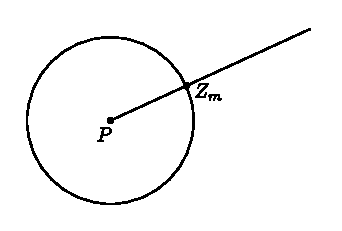
\includegraphics{vol65-figures/fig65-chap4.1.eps}}
\caption{}\label{c5:fig4.1}
\end{figure}

 We introduce $t^m = \dfrac{\delta}{2 | p^m - p |};$ then 
 \begin{equation}
z^m = p + t^m (p^m - p) \tag{4.41}\label{c5:eq4.41}
  \end{equation} 
  and from \eqref{c5:eq4.39}
  \begin{equation}
0 < t^m \leq \frac{1}{2}. \tag{4.42}\label{c5:eq4.42}
\end{equation}
Since $A$ is \textit{strictly monotone} we have 
\begin{equation}
(A(p^m) - A, p^m - p) > (A (p + t (p^m - p)) - A (p), p^m - p)\,\, \forall
  t \in ]0,1[\tag{4.43}\label{c5:eq4.43} 
\end{equation}  
Then, taking $t = t^m$ in \eqref{c5:eq4.43}, we obtain
\begin{equation}
(A(p^m) - A (p), p^m - p) > (A (z^m) - A (p), p^m -p ) > 0.\tag{4.44}\label{c5:eq4.44}
 \end{equation} 
 It follows then from \eqref{c5:eq4.41}, \eqref{c5:eq4.42}, \eqref{c5:eq4.44} that 
 \begin{align}
\begin{cases}
(A(p^m) - A (p), p^m - p) &> \frac{1}{t^m} (A (z^m) - A (p), z^m -
  p)\\ 
  & \qquad \geq 2(A (z^m) - A (p), z^m - p) >\\
&> (A(z^m) - A (p), z^m - p) > 0.\tag{4.45}\label{c5:eq4.45}
\end{cases}
 \end{align}  
 Since\pageoriginale  $S (p, \dfrac{\delta}{2})$ is \textit{compact }
 we can extract from $(z^m)_m$ a subsequence- still denoted $(z^m)_m$-
 such that  
 \begin{equation}
\lim_{m \to + \infty} z^m = z, \in S(p,
\frac{\delta}{2}).\tag{4.46}\label{c5:eq4.46} 
\end{equation}
Since $A$ is continuous it follows from \eqref{c5:eq4.37},
\eqref{c5:eq4.46} that  
\begin{equation}
(A(z) - A(p), z - p ) = 0. \tag{4.47}\label{c5:eq4.47}
\end{equation}

The \textit{strict monotonicity} of $A$ and \eqref{c5:eq4.47} imply
that $z = p$ which is impossible since $| p -z | =
\dfrac{\delta}{2}$. Therefore \eqref{c5:eq4.39} cannot hold
$\Rightarrow \lim\limits_{n \to + \infty} p^n = p$. From the above
properties we can easily prove the following 

\begin{theorem}\label{c5:thm4.2}%theorem 4.2
Assume that $V$and $H$ are finite dimensional and that $(P)$ has a
solution $u$. We suppose that 
\begin{enumerate}[-]
\item $B$  is an injection ,
\item $G$ is convex, proper, l.s.c.,
\item $F = F_0 + F_1 $ with  $F_1$  convex, proper, l.s.c. over  $H$
  and  $F_0$ strictly convex and  $C^1$  over $H$. 
\end{enumerate}
Then $(P) $ has a unique solution and if 
$$
0 < \alpha_0 \leq \rho_n \leq \alpha_1 < 2r
$$
holds, we have for ALG 1 the following convergence properties.
 
  \begin{align*}
& \lim\limits_{n \to + \infty} u^n = u,\\
& \lim\limits_{n \to + \infty} p^n = Bu,\\
& \lim\limits_{n \to + \infty} \lambda^{n+1} - \lambda^n = 0,\\
& \lambda^n \text{ is bounded in }H.
 \end{align*}  
 Moreover if $\lambda$ is a cluster point of $(\lambda^n)_n$, then $\{u , p, \lambda \}$ is saddle point of $\mathscr{L}_r$ over $V \times H  \times H$.
\end{theorem}  

  \subsection{Comment on the use of ALG 1. Further 
  remarks.}\label{c5:ss4.3}%sub sec 4.3
  
  Assume\pageoriginale  that $r$ is \textit{fixed} and what we use a \textit{fixed} value $\rho$ for $\rho_n$. Then from our  computational experience it appears that the best convergence is obtained for $\rho = r$. About the choice of $r$ it can be proved \textit{theoretically} that the \textit{larger} is $r$, the \textit{faster} is the convergence; \textit{practically} the situation is not so simple, for the following reasons:
  
  The \textit{larger} is $r$, the \textit{worst} is the conditioning
  of the optimization problem \eqref{c5:eq3.3} (or of the equivalent
  system \eqref{c5:eq3.5}, \eqref{c5:eq3.6}). Then, since
  \eqref{c5:eq3.3} is \textit{numerically} (and not exactly) solved,
  at each iteration an \textit{error} is made in the determination of
  $\{u^n, p^n \}$. The analysis of this error and the effect of it on
  the global behaviour of ALG 1 is a very complicated problem since we
  have to take into account the conditioning of \eqref{c5:eq3.3}, the
  stopping criterion of the algorithms (usually iterative) solving
  \eqref{c5:eq3.3}, round-off errors, etc $\ldots$.
  
  Fortunately it seems that the combined effect of all these factors
  is an algorithm which is not very sensitive to the choice of $r$
  (see GLOWINSKI - MARROCCO [\ref{k54:e6}], FORTIN-GLOWINSKI
  [\ref{k47:e1}] for more details). 
  
  Form a numerical point of view the only non-trivial part in the use
  of ALG 1 is the solution at each iteration of the above problem
  \eqref{c5:eq3.3}. Taking into account the particular structure of
  \eqref{c5:eq3.3} it follows from CEA-GLOWINSKI [\ref{k29:e1}], and
  CEA [\ref{k27:e2}] that 
  a method very well-suited to the solution of \eqref{c5:eq3.3} is the
  \textit{block relaxation} method described below: 
  
  All the problems \eqref{c5:eq3.3} are of the following type:
  \begin{equation}
\begin{cases}
\mathscr{L}_r (u, p, \mu) \leq \mathscr{L}_r (v, q, \mu)\, \forall \{v,
q \} \in V \times H,\\ 
\{u, p \} \in V \times H, \tag{4.48}\label{c5:eq4.48}
\end{cases}
  \end{equation}
  where $\mu$ is \textit{given}. The minimization problem
  \eqref{c5:eq4.48} is equivalent to the system  
  \begin{align}
&\begin{cases}
&G (v) - G (u) + (\mu, B(v-u)) + r (Bu - p, B(v - u)) \geq 0\, \forall v \in V,\\
&u \in V,\tag{4.49}\label{c5:eq4.49}\\
\end{cases}\\
&\begin{cases}
&F(q) - F (p) -( \mu q-p) + r (p - Bu, q-p) \geq 0\, \forall q \in H,\\
&p \in H. \tag{4.50}\label{c5:eq4.50}
\end{cases}
 \end{align} 
 Then\pageoriginale  a \textit{block relaxation method} for solving \eqref{c5:eq4.49}, \eqref{c5:eq4.50} is 
 \begin{equation}
\{u^0, p^0 \} \text{ given}, \tag{4.51}\label{c5:eq4.51}
 \end{equation}
 \textit{then} $\{u^m, p^m \}$ \textit{known, we obtain} $\{u^{m+1}, p^{m+1} \}$ \textit{from}
 \begin{align}
&\begin{cases}
&G (v) - G(u^{m+1}) + (\mu, B (v-u^{m+1}))\\  
&\hspace{2cm}+ r(Bu^{m+1} - p^m, B (v-u^{m+1})) \geq 0\, \forall v \in V, \\
&u^{m+1} \in V, \tag{4.52}\label{c5:eq4.52}
\end{cases}\\
&\begin{cases}
&F(q) - F(p^{m+1}) - (\mu, q-p^{m+1})\\ 
& \hspace{2cm}+ r(p^{m+1} - Bu^{m+1}, q-p^{m+1}) \geq 0\, \forall q \in H,\\
&p^{m+1} \in H. \tag{4.53}\label{c5:eq4.53}
\end{cases}
\end{align} 

Sufficient conditions for the convergence of
\eqref{c5:eq4.51}--\eqref{c5:eq4.53} may be found in CEA-GLOWINSKI and
CEA, loc. cit. . 

In practice, when using \eqref{c5:eq4.51}--\eqref{c5:eq4.53}, a
stopping test of the following type will be used: 
\begin{equation}
\max (|| u^{m+1} - u^m || , | p^{m+1} - p^m |) \leq
\in.\tag{4.54}\label{c5:eq4.54}   
\end{equation}
 
 Another possibility is to stop after a \textit{fixed number} of
 iterations. If for instance we stop after \textit{only one} iteration
 of \eqref{c5:eq4.51} - \eqref{c5:eq4.53} an if at iteration $n$ of
 ALG 1 we initialise with $\{u^{n-1}, p^{n-1} \}$ the computation of
 $\{u^n, p^n\}$ by \eqref{c5:eq4.51}-\eqref{c5:eq4.53}, then we
 recover ALG 2. 
 
 \begin{remark}\label{c5:rem4.1}%remark 4.1
Other relaxation methods can also be used; moreover it can be
worthwhile to introduce {\em overrelaxation parameters} to increase
the speed of convergence of \eqref{c5:eq4.51} - \eqref{c5:eq4.53}. 
 \end{remark} 
 
 \begin{remark}\label{c5:rem4.2}%remark 4.2
The choice $\rho = r$ may be motivated by the following 
 \end{remark}  
 
\begin{proposition}\label{c5:prop4.1}%proposition4. 1
Suppose\pageoriginale  that $F(q) = \dfrac{1}{2}|q|^2$ and that $G$ is
linear. Then $\forall \lambda^0 \in H$ we have for the sequence
$(u^n)_n $ of ALG1,  convergence to the solution $u$ of $(P)$ in less
than three iterations if we use $\rho_n = \rho = r$, $r$ given.  

{\bf Preliminary remark. } In the above situation we have $(P)$ equivalent to 
\begin{equation}
B^t B u = f 
\end{equation}
where $G(v)= ((f, v)) ~\, \forall v \in  V$.  Therefore using ALG  1 for
solving $(p)$ has no {\em practical} interest.  But even in that
trivial case we shall observe that the behaviour of ALG 1 is
``interesting'' since the convergence of $u^n$ in a {\em finite
  number} of iterations {\em does not imply} a similar convergence for
$p^n$ and $\lambda^n$.  
\end{proposition}

\begin{proof of proposition}\label{c5:prfofprop4.1}%proof of proposition 4. 1
 It follows from \eqref{c5:eq4.17},  \eqref{c5:eq4.18} that in the particular case that we are considering,  ALG 1 reduces to 
\begin{align}
&\lambda^0~~\text{\em given in}~~H, \tag{4.55}\label{c5:eq4.55}\\
&r B^t Bu^n = r B^t p^n - B^t \lambda^n  + f, \tag{4.56}\label{c5:eq4.56}\\
&p^n = \lambda^n + r (Bu^n - p^n), \tag{4.57}\label{c5:eq4.57}\\
&\lambda^{n+1}= \lambda^n + r (Bu^n - p^n). \tag{4.58}\label{c5:eq4.58}
\end{align}
We can easily prove that the unique saddle-point of  $\mathscr{L}_r$ over $V \times H \times H$ is $\{u, Bu, Bu\}$,  i. e.  $p = B u$,  $\lambda = B u$; using the notation $u^{-n}= u^n - u$,  $p^{-n}= p^n - p$,  $\lambda^{-n} = \lambda^n - \lambda$  it follows from \eqref{c5:eq4.56} - \eqref{c5:eq4.58} that 
\end{proof of proposition}
\begin{align}
&B^t \lambda^{-n} + r B ^t (Bu^{-n}-p^{-n}) =0 ~~\forall n \geq 0,  \tag{4.59}\label{c5:eq4.59}\\
&\lambda^{n+1}= p^n,  \Rightarrow \lambda^{-n+1} = p^{-n} ~~\forall n \geq 0,  \tag{4.60}\label{c5:eq4.60}\\
&p^{-n}= \lambda^{-n} + r (Bu^{-n} - p^{-n})~~ \forall n \geq 0. \tag{4.61}\label{c5:eq4.61}
\end{align}
Multiplying\pageoriginale  \eqref{c5:eq4.61} by $B^t$ and comparing with \eqref{c5:eq4.59} we obtain 
\begin{equation}
B^t~ p^{-n}= 0~~ \forall n \geq 0. \tag{4.62}\label{c5:eq4.62}
\end{equation}
Since \eqref{c5:eq4.60},  \eqref{c5:eq4.61} imply 
\begin{equation}
p^{-n+1} = p^{-n} + r (Bu^{- n + 1}-p^{-n+1}) ~~\forall n \geq 0
\tag{4.63}\label{c5:eq4.63} 
\end{equation}
we obtain,  multiplying by $B^t$ and taking account of \eqref{c5:eq4.62}, that 
\begin{equation}
B^t~ Bu^{-n+1} = 0 ~~\forall n \geq 0 \Rightarrow Bu^{- n + 1} = 0
\forall n \geq 0. \tag{4.64}\label{c5:eq4.64} 
\end{equation}

Since$| Bv|$ is a norm on $V$,  \eqref{c5:eq4.64} implies that $u^n =u
~~\forall n \geq 1$.  Hence the convergence of $u^n$ to $u$ requires
at most two iterations.  Using \eqref{c5:eq4.63},  \eqref{c5:eq4.64}
we have  
\begin{equation}
p^{- n + 1} = \frac{1}{1 + r} p^{-n} ~~\forall n \geq 0.
\tag{4.65}\label{c5:eq4.65} 
\end{equation}
It follows from \eqref{c5:eq4.65} that the larger is $r$ the faster
$p^n$ converges to $p = Bu $; for more details on the convergence of
$p^n$ see FORTIN-\break GLOWINSKI [\ref{k47:e1}].  

\section{Convergence of ALG 2}\label{c5:s5}%Sec 5

\subsection{Orientation}\label{c5:ss5.1}%Subsec 5.1

 We shall prove in this section  that under fairly general assumptions on $F$ and $G$we have convergence of ALG 2 if $0 < \rho_n = \rho < \dfrac{1 + \sqrt{5}}{2}r$.  
We do not know if this result is optimal since in some cases ($G$ linear, for example ) the upper bound of the interval of convergence is 2r.  Actually this question is rather academic since in the various experiments we have done with ALG 2,  the optimal choice seems  to be $\rho =r$.  

\subsection{General case}\label{c5:ss5.2}%Subsec 5.2

We study the convergence of ALG 2 with the same hypotheses  of $B$, 
$F$, $G$ as in Sec. \ref{c5:ss4.1}.  We have then  

\begin{theorem}\label{c5:thm5.1}%theorem 5. 1
  We suppose that $\mathscr{L}_r$ has a saddle-point $\{u, p, \lambda\}$ over $V \times H \times H$.  
  Then if the assumptions on $B$, $F$, $G$ are those of 
  Sec.~\ref{c5:ss4.1} and if 
\begin{equation}
0 < \rho_n = \rho < \frac{1 + \sqrt{5}}{2} r, \tag{5.1}\label{c5:eq5.1}
\end{equation}\pageoriginale 
\textit{we have the following convergence properties:}
\begin{align}
& u^n \rightarrow u ~~\text{\em strongly in}~~V, \tag{5.2}\label{c5:eq5.2}\\
& p^n \rightarrow p ~~\text{\em strongly in}~~H,  \tag{5.3}\label{c5:eq5.3}\\
& \lambda^{n+1} - \lambda^n \rightarrow 0 ~~\text{\em strongly in}~~H, \tag{5.4}\label{c5:eq5.4}\\
&\lambda^n~~\text{\em is bounded in}~~H. \tag{5.5}\label{c5:eq5.5}
\end{align}
\end{theorem}
\textit{Moreover if $\lambda^*$ is a weak cluster point of $(\lambda^n)_n$,  then $\{u, p, \lambda\}$  is a saddle-point of $\mathscr{L}_r$ over $V \times H \times H$.}

\begin{proof}
Let us still define $u^{-n}$, $p^{-n}$,  $\lambda^{-n}$ by 
$$
u^{-n} = u^n - u, p^{-n}= p^n - p,  \lambda^{-n} = \lambda^n - \lambda. 
$$
\end{proof}
Since $\{u, p, \lambda\}$ is a saddle-point of $\mathscr{L}_r$ over $V \times H \times H$.  we have 
\begin{align*}
& G(v) - G (u) + (\lambda, B(v - u) ) + r (Bu - p, B(v - u) ) \geq 0~~ \forall 
v \in V, \tag{5.6}\label{c5:eq5.6}\\
& (F'_0(p), q - p) + F_1(q) - F_1(p) - (\lambda,  q - p)\\ 
&\hspace{2cm}+ r(p - Bu, q - p) \geq 0~~ 
\forall q \in H.\tag{5.7}\label{c5:eq5.7}\\
& \lambda =  \lambda + \rho (Bu - p). \tag{5.8}\label{c5:eq5.8}
\end{align*}
Moreover, \eqref{c5:eq3.8}--\eqref{c5:eq3.10} imply 
\begin{align*}
&G (v) - G(u^n) + (\lambda^n, B(v - u^n)) + r (Bu^n - p^{n - 1}, B(v -
  u^n)) \geq 0\, \forall v \in V,\tag{5.9}\label{c5:eq5.9}\\ 
& (F'_0 (p^n),  q - p^n)  + F_1 (q) - F_1(p^n) -(\lambda^n, q - p^n)\\
&  \hspace{3cm}+r (p^n -Bu^n,  q - p^n) \geq \circ\, \forall q \in H,
  \tag{5.10}\label{c5:eq5.10}\\ 
&\lambda^{n+1}= \lambda^n + \rho (Bu^n - p^n). \tag{5.11}\label{c5:eq5.11}
\end{align*}
Taking $v=u^n$ (\resp.  $v=u$) in \eqref{c5:eq5.6} (\resp.
\eqref{c5:eq5.9} ) and $q = p^n$ (\resp.  $q=p$) in \eqref{c5:eq5.7}
(\resp. \eqref{c5:eq5.10}) we obtain\pageoriginale  by addition
\begin{align*}
& r(B\ob{u}^{n } - \ob{p}^{n-1},  B\ob{u}^{n}) +  (\ob{\lambda}^{n}, B
  \ob{u}^{n}) \leq 0, \tag{5.12}\label{c5:eq5.12}\\ 
& (F'_0 (p^n) - F'_0 (p), \ob{p}^{n}) + r (\ob{p}^{n} - B\ob{u}^{n},
  \ob{p}^{n}) - (\ob{\lambda}^{n}, \ob{p}^{n}) \leq
  0. \tag{5.13}\label{c5:eq5.13} 
\end{align*}
By addition of \eqref{c5:eq5.12},  \eqref{c5:eq5.13} it follows that 
\begin{equation}
(F'_0 (p^n) - F'_0 (p), p^n - p) + r | B \ob{u}^{n} - \ob{p}^{n}|^2 +
  (\ob{\lambda}^{n},  B\ob{u}^{n} - \ob{p}^{n})+ r (\ob{p}^{n} -
  \ob{p}^{n - 1}, B\ob{u}^{n}) 
  \leq. \tag{5.14}\label{c5:eq5.14} 
\end{equation}
By subtracting \eqref{c5:eq5.8} from \eqref{c5:eq5.11} we obtain 
\begin{equation}
 |\ob{\lambda}^{n}|^2 - |\ob{\lambda}^{n + 1}|^2 = - 2 \rho (B \ob{u}^{n},
 -\ob{p}^{n}, \ob{\lambda}^{n}) -\rho^2 | B \ob{u}^{n}-
 \ob{p}^{n}|^2. \tag{5.15}\label{c5:eq5.15} 
 \end{equation}
 It follows then from \eqref{c5:eq5.14} ,  \eqref{c5:eq5.15} that 
 \begin{align*}
&|\ob{\lambda}^{n}|^2 - |\ob{\lambda}^{n+1}|^2 \geq 2 \rho (F'_0 (p^n) - F'_0
(p) , \ob{p}^{n}) \\
&\hspace{2cm}+ \rho (2r - \rho) | B \ob{u}^{n}- \ob{p}^{n}|^2 + 2 \rho r
(\ob{p}^{n} - \ob{p}^{n},  B \ob{u}^{n}). \tag{5.16}\label{c5:eq5.16} 
 \end{align*}
 Starting from 
 $$
 B \ob{u}^{n} = (B \ob{u}^{n} - B\ob{u}^{n - 1}) + (B\ob{u}^{n - 1} -
 \ob{p}^{n - 1}) + \ob{p}^{n - 1} 
 $$
 we obtain 
 \begin{align*}
& (B\ob{u}^{n}, \ob{p}^{n} - \ob{p}^{n - 1}) = (B\ob{u}^{n} -
   B\ob{u}^{n- 1}, \ob{p}^{n} -
   \ob{p}^{n - 1})\\ 
  & \hspace{2cm} + (B\ob{u}^{n - 1}, -\ob{p}^{n - 1} - \ob{p}^{n-1}) +
   (\ob{p}^{n-1},  \ob{p}^{n} - \ob{p}^{n-1}). \tag{5.17}\label{c5:eq5.17} 
 \end{align*}
 Since 
 $$
 (\ob{p}^{n - 1}, \ob{p}^{n} - \ob{p}^{n - 1}) = \frac{1}{2} (| \ob{p}^{n}|^2-|
 \ob{p}^{n - 1}|^2 - |\ob{p}^{n} - \ob{p}^{n-1}|^2). 
 $$
 it follows from \eqref{c5:eq5.17} that 
 \begin{equation}
\begin{cases}
2 \rho r (B\ob{u}^{n},  \ob{p}^{n} - \ob{p}^{n - 1}) = & 2 \rho r
(B\ob{u}^{n} - B\ob{u}^{n - 1},  \ob{p}^{n} 
- \ob{p}^{n -1})\\ 
& \quad+ 2 \rho r (B\ob{u}^{n-1} - \ob{p}^{n-1},  \ob{p}^{n}
- \ob{p}^{ n - 1})+ \\ 
& \rho r (|\ob{p}^{n}|^2 - |\ob{p}^{n-1}|^2 - |\ob{p}^{n}- \ob{p}^{n
  -1}|^2).\tag{5.18}\label{c5:eq5.18} 
\end{cases}
 \end{equation} 
 Taking \eqref{c5:eq5.10} ar $n-1$ instead of $n$,  we have 
 \begin{equation}
\begin{cases}
(F'_0 (p^{n-1}),  q - p^{n-1}) + F_1 (q) - F_1 (p^{n - 1}) -
  (\lambda^{n - 1}, q - p^{n-1})+ \\ 
  + r (p^{n-1} - Bu^{n-1},  q - p^{n - 1}) \geq 0. \tag{5.19}\label{c5:eq5.19}
\end{cases}
 \end{equation}\pageoriginale  
 Taking $q = p^{n-1}$ in \eqref{c5:eq5.10} and $q = p^n$ in
 \eqref{c5:eq5.19}  we obtain by addition 
 \begin{equation}
\begin{cases}
(F'_0 (p^n) - F'_0 (p^{n - 1}),  p^n - p^{n-1}) - (\ob{\lambda}^{n} -
  \ob{\lambda}^{n - 1},\\   
 \hspace{3cm} -\ob{p}^{n} - \ob{p}^{n -1}) + r | \ob{p}^{n}- \ob{p}^{n
   -1}|^2 - \\ 
  -r(B \ob{u}^{n} - B \ob{p}^{n -1},  \ob{p}^{n} - \ob{p}^{n-1}) \leq
  0. \tag{5.20}\label{c5:eq5.20} 
\end{cases}
 \end{equation} 
 But since $F'_0$ is \text{monotone}, it follows from \eqref{c5:eq5.20} that 
 \begin{equation}
   r | \ob{p}^{n} - \ob{p}^{n-1}|^2 - (\ob{\lambda}^{n} -
   \ob{\lambda}^{n-1},  \ob{p}^{n}- \ob{p}^{n-1}) 
   -r (B\ob{u}^{n}-B\ob{p}^{n-1}, \ob{p}^{n}- \ob{p}^{n-1}) \leq
   0\tag{5.21}\label{c5:eq5.21} 
 \end{equation} 
 We have (from \eqref{c5:eq3.10}) 
 $$
 \lambda^n = \lambda^{n - 1} + \rho (Bu ^{n - 1 - p^{n-1}})
 $$
 which implies that 
 \begin{equation}
\ob{\lambda}^{n} - \ob{\lambda}^{n - 1}= \rho (B\ob{p}^{n-1} -
\ob{p}^{n - 1}). \tag{5.22}\label{c5:eq5.22} 
 \end{equation} 
 It follows then from \eqref{c5:eq5.21}, \eqref{c5:eq5.22} that 
 $$
 r | \ob{p}^{n} - \ob{p}^{n-1}|^2 - \rho (B\ob{u}^{n-1},  \ob{p}^{n} -
 \ob{p}^{n - 1}) - r 
 (B\ob{u}^{n} - B\ob{u}^{n -1}, \ob{p}^{n} - \ob{p}^{n - 1}) \leq 0
 $$
 i. e. 
 \begin{equation}
r (b u^{-n} - B \ob{u}^{n - 1}, \ob{p}^{n} - \ob{p}^{n - 1}) \geq r | \ob{p}^{n} -
 \ob{p}^{n - 1}|^2 -  
\rho(B\ob{u}^{n - 1} -\ob{p}^{n -1} - \ob{p}^{n}
-\ob{p}^{n-1}). \tag{5.23}\label{c5:eq5.23} 
 \end{equation} 
It' follows then from \eqref{c5:eq5.18} , \eqref{c5:eq5.23} that
\begin{equation}
\begin{cases}
2 \rho r (B\ob{u}^{n}, \ob{p}^{n} -\ob{p}^{n-1}) &\geq  \rho r (|
\ob{p}^{n} |^2 - |\ob{p}^{n-1}|^2 ) +  \rho r | \ob{p}^{n} - \ob{p}^{n-1}|^2 \\  
 & + 2 \rho (r - \rho) (B\ob{u}^{n-1} -\ob{p}^{n-1}, \ob{p}^{n-1},  p^n
  - \ob{p}^{n - 1}). \tag{5.24}\label{c5:eq5.24}
\end{cases}
\end{equation}
Finally,  combining \eqref{c5:eq5.16}, \eqref{c5:eq5.24} we obtain 
\begin{equation}
\begin{cases}
(| \lambda^{-n} |^2 + \rho r |\ob{p}^{n-1}|^2 ) - (|\ob{\lambda}^{n+1}|^2 +
  \rho r | \ob{p}^{n} |^2)  
\geq 2 \rho (F'_0 (P^n) - F'_0 (p), \ob{p}^{n})+ \\
+ \rho (2r - \rho) | B\ob{u}^{n} - \ob{p}^{n} |^2 + \rho r |
\ob{p}^{n} - \ob{p}^{n-1}|^2\\  
\hspace{4cm}+ 2 
\rho (r - \rho) (B\ob{u}^{n-1} - \ob{p}^{n-1},  \ob{p}^{n} - \ob{p}^{n
  - 1}). \tag{5.25}\label{c5:eq5.25} 
\end{cases}
\end{equation}\pageoriginale  
Using the \textit{Schwartz's inequality} it follows from \eqref{c5:eq5.25} that $\forall \alpha > 0$ we have 
{\fontsize{10}{12}\selectfont
\begin{equation}
\begin{cases}
(| \ob{\lambda}^{-n} |^2 + \rho r |\ob{p}^{n-1}|^2 ) - ( |\lambda^{- n
    + 1}|^2 + \rho r  
| \ob{p}^{n} |^2 ) \geq 2 \rho (F'_0 (p^n) - F'_0 (p),  \ob{p}^{n}) +\\
+ \rho (2r - \rho) | B\ob{u}^{n} -\ob{p}^{n}|^2 + \rho r | \ob{p}^{n} -
\ob{p}^{n - 1} |^2 -\rho  
| r - \rho |\\
\hspace{4cm}( \frac{1}{\alpha}| B\ob{u}^{n-1} - \ob{p}^{n - 1}|^2 +
\alpha | \ob{p}^{n}  -\ob{p}^{n -1}|^2). 
\tag{5.26}\label{c5:eq5.26}
\end{cases}
\end{equation}}\relax
It $\rho = r$ it is clear that using the same method as in the proof of 
Theorem 4. 1.  we have \eqref{c5:eq5.2} - \eqref{c5:eq5.5}.  If $0 < 
\rho < r$,  taking $\alpha =1$ and observing that $| r = \rho | = 
r-\rho$,  we observe that we have from \eqref{c5:eq5.26}
\begin{equation*}
\begin{cases}
(|\ob{\lambda}^{n} |^2 + \rho r | \ob{p}^{n - 1}|^2 + \rho (r - \rho)
  B\ob{u}^{n-1}  - \ob{p}^{n - 1}|^2 )\\ 
  \hspace{3cm}- (|\ob{\lambda}^{n+1}|^2 +
  \rho r | \ob{p}^{n}|^2 + \rho (r - \rho) | B \ob{u}^{n} -
  \ob{p}^{n}|^2)\\ 
  \geq 2 \rho (F'_0(p^n) - F'_0 (p),  \ob{p}^{n} ) + \rho r |
  B\ob{u}^{n} - \ob{p}^{n} |^2 + \rho^2| \ob{p}^{n} - \ob{p}^{n-1}|^2 \geq 0.  
\end{cases}
\end{equation*}
which implies clearly \eqref{c5:eq5.2} -\eqref{c5:eq5.5}.  

If $\rho >r$ we have $| r - \rho | = \rho - r $  and then it follows
from \eqref{c5:eq5.26} that \eqref{c5:eq5.2} -\eqref{c5:eq5.5} holds,
if we have $\rho < \rho_M$ where  
\begin{equation*}
\begin{cases}
\rho_M (2r - \rho_M) = \frac{1}{\alpha} \rho_M (\rho_M - r). \\
\rho_M r = \alpha \rho_M (\rho _M - r). \tag{5.27}\label{c5:eq5.27}
\end{cases}
\end{equation*}
By elimination of $\alpha$ it follows from \eqref{c5:eq5.27} that 
$$
\rho^2 _M - r \rho_M - r^2 =0
$$
i. e. (since $\rho_M > 0)$
$$
\rho_M = \frac{1+\sqrt{5}}{2}r. 
$$
Then using basically the same method as in the proof of 
Theorem~\ref{c5:thm4.1} we can easily prove,  from
\eqref{c5:eq5.2}-\eqref{c5:eq5.5},  that $\{u, Bu, \lambda^*\}$ is a
saddle-point of $\mathscr{L}_r$ over $V \times H \times H$ if
$\lambda^*$ is a weak cluster point of $(\lambda^n)_n$.  

\subsection{Finite dimensional case}\label{c5:ss5.3}%Subsec 5.3
Using\pageoriginale   a variant of the proof of Theorem~\ref{c5:thm5.1},  and 
Lemma~\ref{c5:lem4.1}, we can easily prove 

\begin{theorem}\label{c5:thm5.2}%theorem 5. 2
Assume that the assumptions  on $V$, $H$, $F$, $B$, $G$ are those of 
the statement of Theorem \ref{c5:thm4.2}.  Then if
$$ 
0 < \rho_n = \rho < \frac{1+ \sqrt{5}}{2}r
$$
the conclusions of the statement of Theorem \ref{c5:thm4.2} still hold.  
\end{theorem}

\subsection{Comments on the choice of $\rho$ and $r$}\label{c5:ss5.4}

\subsubsection{Some remarks}\label{c5:sss5.4.1}

\begin{remark}\label{c5:rem5.1}%remark 5. 1
 If $G$ is linear  it has been proved by GABAY-MERCIER [1] that ALG 2 converges if 
 $$
 0 < \rho_n = \rho < 2 r. 
 $$
\end{remark}

The proof of this result is rather technical and an open question is to decide if it can be extended to the more general cases we have considered in these notes.
 
\begin{remark}\label{c5:rem5.2}%remark 5. 2
If $G$ is is linear we observe that the step \eqref{c5:eq3.8} of ALG 2 is a \textit{linear problem}  related to the \textit{self adjoint operator}$B^t B$.  Therefore in the finite dimensional case, assuming $B$ injective,  it will be convenient to \textit{factorize}(by a Cholesky method, for example) the \textit{symmetric, positive definite} matrix$B^tB$ once and for all,  before starting the iterations of ALG 2. 
\end{remark}

\subsubsection{On the choice of $\rho$ and $r$}\label{c5:sss5.4.2}

If $r$ is given our computational experience seems to indicate that
the best choice for $\rho$ is $\rho =r$.  The choice of $r$ is  not
clear  and ALG 2 appears to be \textit{more sensitive} to the choice
of $r$ than ALG 1. By the way, ALG 1 seems to be more robust on
\textit{very stiff} problem 
than ALG 2; we mean that the choice of the parameter is less critical
and that the \textit{computational time} with ALG  1 may become
\textit{much shorter} than with ALG 2.  

\begin{remark}\label{c5:rem5.3}%remark 5. 3
 We have seen\pageoriginale   in Remark \ref{c5:rem4.2} that if $F (q) = \dfrac{1}{2} | q |^2$ and $G$ is linear, the sequence $\{ u^n \}_n$ related to ALG 1 converges in two iterations (at most) if we use $\rho = r$. If we use ALG  2 with the same hypotheses on $F$, $G$ then we have convergence of $\{ u^n \}_n$ in two iterations at  most, only if $\rho = r =1$ (for any choice of $\{ p^0, \lambda^1 \}$). This fact also confirms the greater robustness of ALG 1.  
\end{remark}

\section{Applications}\label{c5:s6}%6

\subsection{Bingham flow in a cylindrical pipe}\label{c5:ss6.1}%subsec 6.1.

It is the problem considered in CH. 2,  Sec. 6 and also in Sec. 1. 1 of this Chapter (we recall that $\Omega$ is a \textit{bounded} domain of $\mathbb{R}^2$):
\begin{equation}
\min_{v \in H^1_0 (\Omega)} \left\{\frac{\nu}{2} \int_\Omega | \nabla
v |^2 dx + g \int_\Omega | \nabla v | dx - \int_\Omega fv dx
\right\}. \tag{6.1}\label{c5:eq6.1} 
\end{equation}
Then \eqref{c5:eq3.1} is a particular $(P)$ problem corresponding to 
\begin{align*}
&V = H^1_0 (\Omega),  H = L^2 (\Omega ) \times L^2 (\Omega ), B =
  \nabla, \tag{6.2}\label{c5:eq6.2}\\ 
&F (q) = \frac{\nu}{2}\int_\Omega | q |^2 ~ dx + g \int_\Omega | q |
  dx, \tag{6.3}\label{c5:eq6.3} \\ 
&G (v) = -\int_\Omega ~ fv ~ dx. \tag{6.4}\label{c5:eq6.4}
\end{align*}
Moreover we have $F = F_0 + F_1$ with 
\begin{align*}
F_0 (q) &= \frac{\nu}{2}\int_\Omega | q|^2 dx ,  F'_0 (q) = \nu q,
\tag{6.5}\label{c5:eq6.5}\\ 
F_1 (q) &=g \int_\Omega |q| dx . \tag{6.6}\label{c5:eq6.6}
\end{align*}
it follows then from \eqref{c5:eq6.2} -\eqref{c5:eq6.6} that the various assumptions required to apply 
Theorem \ref{c5:thm4.1} and \ref{c5:thm5.1} are satisfied.  Therefore we 
can solve \eqref{c5:eq6.1} by ALG 1 and ALG 2.  Moreover since $G$ is 
linear the GABAY-MERCIER[\ref{k48:e1}] result holds (see Remark \ref{c5:rem5.1}) and ALG 2  converges if $0 < \rho_n = \rho < 2r$.  The augmented  Lagrangian $\mathscr{L}_r$  to be used in this case is given by 
\begin{equation}
\begin{cases}
\mathscr{L}_r (v, q, \mu) &=\frac{\nu}{2} \int_\Omega |q|^2 dx + g \int_\Omega fv dx + \int_\Omega \mu \cdot (\nabla v-q) dx \\
&+ \frac{r}{2} \int_\Omega | \nabla v-q|^2 dx. \tag{6.7}\label{c5:eq6.7}
\end{cases}
\end{equation}
\textbf{\em Solution\pageoriginale   of \eqref{c5:eq6.1} by ALG 1.}

When applying ALG 1 to  the solution of \eqref{c5:eq6.1} it follows
from \eqref{c5:eq3.2}-\eqref{c5:eq3.4}, \eqref{c5:eq6.7} that we have  
\begin{equation}
\lambda^0 \in L^2 (\Omega) \times L^2 (\Omega), 
\text{arbitrarily given, }\tag{6.8}\label{c5:eq6.8}
\end{equation}
\textit{then for }$n\geq 0$, 
\begin{equation}
\begin{cases}
-r\Delta u^n &= f + \nabla \cdot \lambda^n - r \nabla \cdot p^n \text{on} 
\Omega, \\
u^n |_\Gamma &= 0, \tag{6.9}\label{c5:eq6.9}
\end{cases}
\end{equation}

\begin{equation}
\begin{cases}
p^n (x) &= 0 (\text{if} g \ge | \lambda^n 9x) + r \nabla u^n (x) |, \\
p^n (x) &= \dfrac{\lambda^n (x) + r \nabla u^n (x)}{\nu + r} \left(1- \dfrac{g}
{|\lambda^n (x) + r \nabla u^n (x) |}\right) \text{elsewhere, } 
\tag{6.10}\label{c5:eq6.10}
\end{cases}
\end{equation}

\begin{equation}
\begin{cases}
\lambda^{n+1} = \lambda^n + \rho_n (\nabla u^n - p^n). 
\tag{6.11}\label{c5:eq6.11}
\end{cases}
\end{equation}

\noindent \textbf{Solution of \eqref{c5:eq6.1} by ALG}

We have to replace \eqref{c5:eq6.8} by
\begin{equation}
\{ p^0, \lambda^1 \} \text{arbitrarily given in} (L^2 (\Omega ))^2 \times 
(L^2 (\Omega ))^2, \tag{6.12}\label{c5:eq6.12}
\end{equation}
and \eqref{c5:eq6.9} by 
\begin{equation}
\begin{cases}
-r \Delta u^n = f + \nabla \cdot \lambda^n - r \nabla p^{n-1}
\text{on}\Omega. \\ 
u^n |_\Gamma = 0. \tag{6.13}\label{c5:eq6.13}
\end{cases}
\end{equation}

\begin{remark}\label{c5:rem6.1}%remark 6. 1
 In practice \eqref{c5:eq6.8}--\eqref{c5:eq6.11} and 
 \eqref{c5:eq6.12}, \eqref{c5:eq6.13}, \eqref{c5:eq6.10},\break 
 \eqref{c5:eq6.11} will be applied to {\em finite  element} or {\em 
 finite difference} approximations of \eqref{c5:eq6.1}. It follows then 
 from \eqref{c5:eq6.9}, \eqref{c5:eq6.13} that it is easy to use either 
 ALG 1 (combined with the {\em block relaxation method} of 
 Sec.~\ref{c5:ss4.3}) or ALG 2, once we have at our disposal an 
 efficient program for solving approximate Dirichlet problems for $-\Delta$.  
\end{remark}

\noindent
\textbf{Bibliographical comments.}\pageoriginale   Numerical solutions
of \eqref{c5:eq6.1} by ALG 1 and ALG 2 may be found in GABAY-MERCIER
[\ref{k48:e1}, GLOWINSKI-MARROCCO [\ref{k54:e3}]; we can also find in
  FORTIN [\ref{k46:e2}] and 
  iterative method of solution of \eqref{c5:eq6.1},  close to ALG 2
  but obtained by a different approach.  

\subsection{Elastic-plastic torsion of a cylindrical 
bar}\label{c5:ss6.2}%sec

It is the problem of Chap.~\ref{chap2},  Sec.~\ref{c2:s3},  also considered in 
Sec.~1.1 ($\Omega$ is a bounded domain of $\mathbb{R}^2$ in the sequel):
\begin{equation}
\min _{v \in K}[\frac{1}{2} \int_\Omega | \nabla v |^2 dx - 
\int_\Omega fv dx ],  \tag{6.14}\label{c5:eq6.14} 
\end{equation}
where \qquad $K= \{ v | v \in H^1_0 (\Omega ), | \nabla v| \leq 1a. e. \}$;
\eqref{c5:eq6.14} is a particular $(P)$ problem corresponding to 
\begin{align*}
&V = H^1_0 (\Omega ) ,  H = L^2 (\Omega ) \times L^2 (\Omega ), B = 
\nabla, \tag{6.15}\label{c5:eq6.15}\\ 
&G (V) = - \int_\Omega fv ~ dx, \tag{6.16}\label{c5:eq6.16}\\
&F = F_0 + F_1,  \tag{6.17}\label{c5:eq6.17}
\end{align*}
where 
\begin{align*}
&F_0 (q) = \frac{1}{2}\int_\Omega | q |^2 dx \Rightarrow F'_0 (q) = q, \tag{6.18}\label{c5:eq6.18}\\
&F_1 (q) = L_{\hat{K}} (q) \tag{6.19}\label{c5:eq6.19}
\end{align*}
with $\hat{K} = \{q \in H,  | q | \leq 1 a. e. \}$ and $\L_{\hat{K}}$ the  \textit{indicator functional} of $\hat{K}$ i.e.  
\begin{equation}
L_{\hat{K}} (q) = 
\begin{cases}
0 &\text{ if } q \in \hat{K}, \\
+ \infty &\text{ if } q \notin\hat{K}. \tag{6.20}\label{c5:eq6.20}
 \end{cases} 
 \end{equation}
 Here too, it follows from \eqref{c5:eq6.15} - \eqref{c5:eq6.20} that 
 the various assumptions required to apply Theorem \ref{c5:thm4.1} and 
 \ref{c5:thm5.1} are satisfied.  Therefore we can solve 
 \eqref{c5:eq6.14} by ALG 1  and  ALG 2.  Moreover from the linearity 
 of $G$ we have the convergence of ALG 2 if $0 < \rho_n = \rho < 2r$. 
 In the present case $\mathscr{L}_r$ is given by    
 \begin{align*}
\mathscr{L}_r (v, q, \mu ) &= \frac{1}{2} \int_\Omega | q |^2 dx + 
I_{\hat{K}} (q) - \int_\Omega fv ~ dx\\ 
&\hspace{1cm}+ \int_\Omega \mu \cdot 
(\nabla v-q) dx + \frac{r}{2} \int_\Omega | \nabla v-q 
|^2 dx.  \tag{6.21}\label{c5:eq6.21}   
 \end{align*}\pageoriginale   
 
\medskip
\noindent
 \textbf{Solution of \eqref{c5:eq6.1} by ALG 1.}
 
It follows from \eqref{c5:eq3.2}--\eqref{c5:eq3.4}, \eqref{c5:eq6.21} 
that when applying ALG 1 to \eqref{c5:eq6.14} we obtain  
 
\begin{equation}
\lambda^0 \text{arbitrarily given in} (L^2(\Omega ))^2,  
\tag{6.22}\label{c5:eq6.22} 
 \end{equation} 
 \textit{then for $n\geq0, $}
 \begin{equation}
\begin{cases}
-r \Delta u^n = f + \Delta \cdot \lambda^n - r \nabla \cdot p^n 
~\text{on}~\Omega,\\ 
u^n | _\Gamma = 0, \tag{6.23}\label{c5:eq6.23}
\end{cases}
 \end{equation} 
 \begin{align*}
&p^n = \frac{\lambda^n + r \nabla u^n}{\underline{\sup} (1 + r, 
| \lambda^n + r u^n |)}, \tag{6.24}\label{c5:eq6.24}\\ 
&\lambda^{n + 1} = \lambda^n + \rho_n (\nabla u^n - p^n). 
\tag{6.25}\label{c5:eq6.25} 
\end{align*} 

\noindent \textbf{Solution of \eqref{c5:eq6.1} by ALG}

We have to replace \eqref{c5:eq6.22} by \eqref{c5:eq6.21} and 
\eqref{c5:eq6.23} by \eqref{c5:eq6.13}. Still applies to 
\eqref{c5:eq6.14} and numerical solutions of (6. ) by ALG 1,  ALG 2 may 
be found in GLOWINSKI-MARROCCO [\ref{k54:e3}],  GABAY-MERCIER
[\ref{k48:e1}].     
 
\subsection{A nonlinear Dirichlet problem}\label{c5:ss6.3}%sec 6.3.
 
 We follow in this section GLOWINKSKI-MARROCCO [\ref{k54:e6}]; Let us
 consider $1 < s < + \infty$ and  
 $$
 W^{1, s}_0,(\Omega ) = \overline{\mathscr{D}(\Omega)} W^{1, s}
 (\Omega) = \{v \in  W^{1, s} (\Omega ),  v |_\Gamma = 0 \},  
 $$
 where $\Omega$ is a \textit{bounded} domain of $\mathbb{R}^N$.  
 
 Then we consider on $\Omega$ the following nonlinear Dirichlet problem: 
\begin{equation}
\begin{cases}
- \nabla \cdot (|\nabla u |^{s-2}\nabla u) = f, \\
u|_\Gamma = 0, \tag{6.26}\label{c5:eq6.26}
\end{cases}
\end{equation}
where\pageoriginale $f \in V' = W^{-1,  s'}(\Omega ) (\frac{1}{s} +
\frac{1}{s'}  
= 1 \Rightarrow s' = \frac{s}{s-1})$.  it can be proved (see,  for 
instance GLOWINKSI-MARROCCO [\ref{k54:e6}]) that \eqref{c5:eq6.26} has a unique 
solution which is also the solution of    
\begin{equation}
\min_{v \in W^{1, s}_0 (\Omega )} \left[\frac{1}{s}\int_\Omega 
|\nabla v |^s dx - < f,  v > \right]. \tag{6.27}\label{c5:eq6.27} 
\end{equation}
We observe that $W^{1, s}_0 (\Omega )$ \textit{is not an Hilbert space} 
if $s \neq 2$, therefore we cannot apply Theorems 4.1 and 5.1 to the 
iterative solution of \eqref{c5:eq6.27}. Nevertheless once 
\eqref{c5:eq6.27} has been approximated by a convenient finite element 
or finite difference method it is possible to apply the above theorems 
(or Theorems \ref{c5:thm4.2}, \ref{c5:thm5.2}) to the iterative solution of the approximate 
problem. For the sake of simplicity we shall confine our study to the 
continuous problem, since it has simpler notation. We have        
\begin{align*}
&V= W^{1, s}_0(\Omega ),  H = (L^s (\Omega ))^N ,  H' = (L^{s'}(\Omega
  ))^N,  B = \nabla,  \\ 
&F (q) = F_0 (q) = \frac{1}{s}\int_\Omega |q|^s dx,  F' (q) =
  q|q|^{s-2}, \\ 
& G(v) =  < f,  v >. 
\end{align*} 
We observe that 
$$
\lim_{|q|_s \to + \infty }\frac{F(q)}{|q|_s}= + \infty,  
$$
where 
$$
|q|_s = (\int_\Omega  | q|^s dx ) ^{1/s}= ||q||_{(L^s (\Omega)}^N. 
$$
We also have $\forall p$, $q \in H$: 
\begin{align*}
&(F'(q) - F'(p), q - p) \geq \alpha |q-p|^s_s ~\text{ if }~ s\geq 2,
  \tag{6.28}\label{c5:eq6.28}\\ 
&(F'(q) - F'(p), q - p) \geq \alpha \frac{|q-p|^2_s}{(|p|_s+ |q|_s
    )^{2-s}} \text{ if }1  < s \leq 2,  \tag{6.29}\label{c5:eq6.29}\\ 
&|F'(q)-F'(p) |_{s'} \geq \beta (|p|_s + |q|_s )^{s-2}|q-p|_s  \text{
    if } s \leq 2, \tag{6.30}\label{c5:eq6.30}\\ 
&|F' (q) - F'(p) |_{s'} \geq \beta |q-p|^{s-1}_s \text{ if } 1 < s
  \leq 2, \tag{6.31}\label{c5:eq6.31} 
\end{align*}
where $\alpha$, $\beta$ are independent of $p$, $q$ and are strictly
positive.  

\begin{exercise}\label{c5:exer6.1}%exercise 6. 1
 Prove\pageoriginale   \eqref{c5:eq6.28} - \eqref{c5:eq6.31}. 
\end{exercise}

We refer to GLOWINSKI - MARROCCO [\ref{k54:e6}] for a detailed
analysis, including error estimates, of a finite element approximation
of \eqref{c5:eq6.26}, \eqref{c5:eq6.27} (see also CIARLET [\ref{k31:e2}]).  

From our numerical experience it appears that solving 
\eqref{c5:eq6.26}, \eqref{c5:eq6.27} if $s$ is close to 1 (say $1 < s 
<1. 3$) or large (say $s >5$ ) is a very difficult task  if one uses 
standard iterative methods; to our knowledge the only very efficient 
methods are ALG 1 and ALG 2  (or closely related algorithms; see 
GLOWINSKI-MARROCCO, loc.  cit.,  for more details).  The augmented 
Lagrangian $\mathscr{L}_r$ to used for solving \eqref{c5:eq6.26}, 
\eqref{c5:eq6.27} is defined by         
\begin{equation}
\mathscr{L}_r (v, q, \mu ) = \frac{1}{s} \int_\Omega |q|^s dx  - <f, v> 
+ \frac{r}{2}\int_\Omega | \nabla v-q|^2 dx + \int_\Omega \mu 
\cdot (\nabla v-q) dx.  \tag{6.32}\label{c5:eq6.32}  
\end{equation}

\noindent
\textbf{Solution of \eqref{c5:eq6.1} by ALG 1.}

It follows from \eqref{c5:eq3.2}--\eqref{c5:eq3.4}, \eqref{c5:eq6.32} 
that when applying ALG 1 to \eqref{c5:eq6.6}, \eqref{c5:eq6.27} we obtain  
\begin{equation}
\lambda^0 \in (L^{s'} (\Omega ))^N, \tag{6.33}\label{c5:eq6.33}
\end{equation}
\textit{then for $n\geq 0$}
\begin{equation}
\begin{cases}
-r\Delta u^n = f + \nabla \cdot \lambda^n - r \nabla 
\cdot p^n \text{ in }\Omega, \\ 
u^n |_\Gamma = 0,\tag{6.34}\label{c5:eq6.34}
\end{cases}
\end{equation}
\begin{align*}
&|p^n|^{s-2}p^n+ rp^n = r \nabla u^n + \lambda^n, \tag{6.35}\label{c5:eq6.35}\\
&\lambda^{n+1} = \lambda^n + \rho_n (\nabla u^n
  -p^n). \tag{6.36}\label{c5:eq6.36} 
\end{align*}
The nonlinear  system \eqref{c5:eq6.34} , \eqref{c5:eq6.35} can be 
solved by the block relaxation method of Sec.~\ref{c5:ss4.3} and we observe 
that if $u^n$ and $\lambda^n$ are known  (or estimated) in 
\eqref{c5:eq6.35} the computation of $p^n$ is an easy task since 
$|p^n|$ is solution of the single variable nonlinear equation     
\begin{equation}
|p^n|^{s-1} + r |p^n| = | r \nabla u^n + \lambda^n | 
\tag{6.37}\label{c5:eq6.37} 
\end{equation}\pageoriginale  
which can be easily solved by various methods; once $| p^n |$ is known, 
we obtain $p^n$ by solving a trivial linear equation (in $(L^s (\Omega ))^N)$.  

\noindent \textbf{Solution of \eqref{c5:eq6.26}, \eqref{c5:eq6.27} by ALG 2.} 

We have to replace \eqref{c5:eq6.33} by 
\begin{equation}
\{ p^0 , \lambda^1 \} \in H \times H' \tag{6.38}\label{c5:eq6.38}
\end{equation}
and \eqref{c5:eq6.34} by 
\begin{equation}
\begin{cases}
-r \Delta u^n = f + \nabla \cdot \lambda^n - r \nabla 
\cdot p^{n-1}\\ 
u^n |_\Gamma =0. \tag{6.39}\label{c5:eq6.39}
\end{cases}
\end{equation}

Remark \ref{c5:rem6.1} 
 still applies to \eqref{c5:eq6.26}, \eqref{c5:eq6.27} and since $G$ is 
 linear we can take $0 < \rho_n = \rho < 2r$ if we are using ALG 2.  
 For more details and comparisons with other methods see 
 GLOWINSKI-MARROCCO [\ref{k54:e3}], [\ref{k54:e6}], [\ref{k54:e8}].    


\begin{remark}\label{c5:rem6.2}%remark 6. 2
ALG 1 and ALG 2 have also been successfully applied to the iterative 
solution of \textit{magneto-static} problems (see GLOWINSKI-MARROCCO 
[\ref{k54:e7}]). They have also been applied  by  GLOWINSKI-\break MARROCCO
[\ref{k54:e3}]  to the 
solution of the \textit{subsonic flow} problem described in 
Ch.~\ref{chap4}.  Sec.~\ref{c4:s3}; in this last case using ALG 1 and 
ALG 2 we obtain easy variants of  
\eqref{c5:eq6.33}-\eqref{c5:eq6.36} and \eqref{c5:eq6.38}, 
\eqref{c5:eq6.39},  \eqref{c5:eq6.35}, \eqref{c5:eq6.36}.         
 \end{remark}
 
\subsection{Application to the solution of mildly nonlinear 
systems}\label{c5:ss6.4}

Let $\A\limits_\sim$ be $N\times N$  symmetric, positive definite 
matrix $\D\limits_\sim$ a diagonal,  positive semi-definite matrix, and 
$\f\limits_\sim \in \mathbb{R}^n$. Let $\phi : \mathbb{R}\to 
\mathbb{R}$ be a $C^0$ and nondecreasing functions (we can always  
suppose that $\phi (0) = 0)$.  Using the same notation as in 
Chapter~\ref{chap4},  Sec.~\ref{c4:s2}.,  we associate to 
$\ve\limits_\sim = \{v_1v_2\dots v_N \}  
 \in \mathbb{R}^N$ the vector $\phi (\ve\limits_\sim) \in 
 \mathbb{R}^N$ defined by        
\begin{equation}
(\phi (\ve\limits_\sim ))_i = \phi (v_i)\, \forall i = 1, \ldots. N. 
\tag{6.40}\label{c5:eq6.40} 
\end{equation}
Then\pageoriginale   we consider the \textit{nonlinear system}
\begin{equation}
\A\limits_\sim \uu \limits_\sim \D\limits_\sim \phi (\uu\limits_\sim ) 
= \f\limits_\sim. \tag{6.41}\label{c5:eq6.41} 
\end{equation}
In Chapter \ref{chap4},  Sec.~\ref{c4:ss2.6}, various methods for 
solving \eqref{c5:eq6.41} have been given,  but in this section we 
would  like to show that \eqref{c5:eq6.41} can also be solved by ALG1,  
ALG2,  once a convenient augmented Lagrangian has been introduced.    

\begin{remark}\label{c5:rem6.3}%remark 6. 3
The methods to be described later are easily generalized to the case 
where $\A \limits_\sim$ is {\em not symmetric but still positive definite.} 

Let us define
$$
\phi (t) = \int^t_0 \phi (\tau ) d \tau. 
$$
\end{remark}
Since $\phi$ is $C^0$ and nondecreasing we have that $\phi $ is $C^1$ 
and \textit{convex}. It follows then from the symmetry of $A$ that 
solving \eqref{c5:eq6.41} is equivalent to solving the minimization 
problem   
\begin{equation}
\begin{cases}
J(\uu\limits_\sim ) \leq J (\ve\limits_\sim )\, \forall \ve \in \mathbb{R}^N, 
u \in \mathbb{R}^N.\\
  u \in \mathbb{R}^N
\end{cases} \tag{6.42}\label{c5:eq6.42}
\end{equation}
In \eqref{c5:eq6.42} we have 
\begin{equation}
J(\ve\limits_\sim) = \frac{1}{2} ({\A\limits_\sim} \ve\limits_\sim, \ve\limits_\sim) 
+ \sum^N_{i=1} ~ d_i \phi (v_i) - (\f\limits_\sim, \ve\limits_\sim ), 
\tag{6.43}\label{c5:eq6.43}  
\end{equation}
where $(\cdot , \cdot)$ denotes the usual inner-product of 
$\mathbb{R}^N$ and $|| \cdot ||$ the corresponding norm and where  
$$
\D\limits_\sim= 
\begin{pmatrix}
d_{1 \ddots} & &0\\
 & d_{i\ddots} &\\
0 & &d_N
\end{pmatrix}
$$

From the above properties of $\A\limits_\sim$, $\D\limits_{\sim\sim}$ 
and $\Phi$ it follows from e. g. CEA [\ref{k27:e1}], [\ref{k27:e2}]
that \eqref{c5:eq6.41},  
\eqref{c5:eq6.42} has a \textit{unique solution.}  

\begin{remark}\label{c5:rem6.4}%remark 6. 4
 If fact \eqref{c5:eq6.41} has a unique solution if $\A\limits_\sim$ is 
 {\em positive definite, possibly not symmetric},  the assumption  on 
 $\phi$ and $\D\limits_\sim$ remaining the same.   
\end{remark}


The\pageoriginale   problem \eqref{c5:eq6.42} is a particular problem $(P)$ corresponding to 
\begin{align*}
&V = H = \mathbb{R}^N,  B = I, \tag{6.44}\label{c5:eq6.44}\\
&G (\ve\limits_\sim ) = \sum^N_{i=1} ~ d_i \Phi (v_i) - 
(\f\limits_\sim, \ve\limits_\sim ), \tag{6.45}\label{c5:eq6.45}\\ 
&F (\q\limits_\sim )  = F_0 (\q\limits_\sim ) = \frac{1}{2} ( 
\A\limits_\sim \q\limits_\sim \q\limits_\sim ) \Rightarrow F'_0 
(\q\limits_\sim ) = \A\limits_\sim \q\limits_\sim. 
\tag{6.46}\label{c5:eq6.46}   
\end{align*}
From these properties we can solve \eqref{c5:eq6.41}, \eqref{c5:eq6.42} 
by using ALG 1 and ALG 2 (we observe that unlike in the above examples 
$G$ is nonlinear).   

\begin{remark}\label{c5:rem6.5}%remark 6. 5
Instead of using $G$ and $F$ defined by \eqref{c5:eq6.44}, 
\eqref{c5:eq6.45},  we can use  
 \begin{align*}
G (v)  &= \sum^N_{i=1} ~ d_i \Phi (v_i), \\
F (q) &= \frac{1}{2} (\A\limits_\sim \q\limits_\sim , \q\limits_\sim ) 
- (\f\limits_\sim , \q\limits_\sim ).  
 \end{align*} 
\end{remark}

\noindent
The augmented Lagrangian to be associated with 
\eqref{c5:eq6.44}--\eqref{c5:eq6.46} is  
\begin{equation}
\mathscr{L}_r (\ve\limits_\sim, \q\limits_\sim\uu\limits_\sim ) = 
\frac{1}{2} (\A\limits_\sim \q\limits_\sim \q\limits_\sim ) + 
\sum^N_{i=1} d_i \Phi (v_i) - (\f\limits_\sim,  \ve \limits_\sim ) + 
\frac{r}{2}||\ve\limits_\sim-\q\limits_\sim ||^2 + (\underset{\sim}\mu, 
 \ve\limits_\sim -\q\limits_\sim ). \tag{6.47}\label{c5:eq6.47}     
\end{equation}
Since the constraint $\ve\limits_\sim$, $\q\limits_\sim = 0$ is linear 
we know that $\mathscr{L}_r$  has a saddle-point over 
$\mathbb{R}^N\times \mathbb{R}^N \times \mathbb{R}^N$; actually this 
saddle-point is unique and is equal to $\{ \uu\limits_\sim, 
\uu\limits_\sim,  \A\limits_\sim \uu\limits_\sim \}$.      

\noindent
\textbf{Solution of \eqref{c5:eq6.41} by ALG 1}

It follows from \eqref{c5:eq3.2}-\eqref{c5:eq3.4}, \eqref{c5:eq6.47} 
that when applying ALG 1 to \eqref{c5:eq6.41}, \eqref{c5:eq6.42} we 
obtain   
 \begin{equation}
\underset{\sim}\lambda^0 \in \mathbb{R}^N, \tag{6.48}\label{c5:eq6.48}
 \end{equation} 
 \textit{then for $n \geq 0$},
 \begin{align*}
&r {\uu\limits_\sim}^n + \D\limits_\sim \phi ({\uu\limits_\sim}^n ) = 
\f\limits_\sim + r {\p\limits_\sim}^n -\mathop{\lambda}_\sim {}^n, 
\tag{6.49}\label{c5:eq6.49}\\  
&( r\I\limits_\sim + \A\limits_\sim ) {\p\limits_\sim}^n = r 
{\uu\limits_\sim}^n + \mathop{\lambda}_\sim {}^n, 
\tag{6.50}\label{c5:eq6.50}\\  
&\underset{\sim}\lambda^{n+1} = \underset{\sim}\lambda^n + \rho_n 
({\uu\limits_\sim}^n - {\p\limits_\sim}^n ). \tag{6.51}\label{c5:eq6.51}   
 \end{align*} 
The nonlinear\pageoriginale   system \eqref{c5:eq6.49}, \eqref{c5:eq6.50} can be solved 
by the \textit{block relaxation} method of Sec. \ref{c5:ss4.3} and we 
observe that if ${\p\limits_\sim}^n$ and $\underset{\sim}\lambda^n$ are 
known (or estimated) in \eqref{c5:eq6.49} the computation of 
${\uu\limits_\sim}^n$  is easy since it is reduced to the solution of $N$ 
\textit{independent, single variable nonlinear equations} of the 
following type      
\begin{equation}
r \xi + d \phi (\xi ) = b ~(\text{ with }d \geq 0). \tag{6.52}\label{c5:eq6.52}
\end{equation}
Since $r >0$ and $\phi$ is $C^0$  and non decreasing,
\eqref{c5:eq6.52} has  a unique solution which can be computed by
various standard method (see, e.g.,  HOUSEHOLDER [\ref{k57:e1}],
BRENT[\ref{k13:e1}]).
Similarly if ${\uu\limits_\sim}^n$ and $\underset{\sim}\lambda^n$ are
known is \eqref{c5:eq6.50} we obtain ${\p\limits_\sim}^n$ by solving a
linear system whose matrix is $r$ is independent of $n$ it is very
convenient to prefactorize $r \I\limits_\sim + \A\limits_\sim$ (by
Cholesky or Gauss methods).  

\noindent \textbf{Solution of \eqref{c5:eq6.1} by ALG 2.}

We have to replace \eqref{c5:eq6.48} by 
\begin{equation}
\left\{ \p\limits_\sim^0, \underset{\sim}\lambda^1 \right\} \in
\mathbb{R}^N \times \mathbb{R}^N \tag{6.53}\label{c5:eq6.53} 
\end{equation} 
and \eqref{c5:eq6.49} by
\begin{equation}
r \uu\limits_\sim^n + \D\limits_\sim \phi (\uu\limits_\sim^n ) = \f 
\limits_\sim + r \p\limits_\sim^{n-1} - \underset{\sim}\lambda^n. 
\tag{6.54}\label{c5:eq6.54}  
 \end{equation} 
It follows from Theorem \ref{c5:thm5.2} that we have convergence of 
\eqref{c5:eq6.53}, \eqref{c5:eq6.54}, \eqref{c5:eq6.50}, 
\eqref{c5:eq6.51} if $0   
< \rho_n = \rho <\dfrac{1 + \sqrt{5}}{2}r$. 

\begin{remark}\label{c5:rem6.6}%remark 6. 6:
Suppose that $\rho_n = \rho = r$ in ALG 2; we have then
\begin{equation}
\begin{cases}
r \uu\limits_\sim^n + \D\limits_\sim \phi (\uu\limits_\sim^n ) = \f\limits_\sim + r \p\limits_\sim^{n-1} - \underset{\sim}\lambda^n, \\
r\p\limits_\sim^n + \A\limits_\sim \p\limits_\sim^n = r \uu\limits_\sim^n + \underset{\sim}\lambda^n, \\
\underset{\sim}\lambda^{n+1} = \underset{\sim}\lambda^n + r 
(\uu\limits_\sim^n - \p\limits_\sim^n ). \tag{6.55}\label{c5:eq6.55} 
\end{cases}
\end{equation} 
\end{remark}
It follows from \eqref{c5:eq6.55} that 
\begin{equation}
\underset{\sim}\lambda^{n+1} =  \A\limits_\sim \p\limits_\sim^n, 
\tag{6.56}\label{c5:eq6.56} 
\end{equation}
Then\pageoriginale   from \eqref{c5:eq6.55}, \eqref{c5:eq6.56} we obtain 
\begin{align*}
&r \uu\limits_\sim^n + \D\limits_\sim\phi (\uu\limits_\sim^n ) + 
\A\limits_\sim \p\limits_\sim^{n-1} = \f\limits_\sim + r 
\p\limits_\sim^{n-1}, \tag{6.57}\label{c5:eq6.57}\\  
& r \p\limits_\sim^n + \A\limits_\sim \p\limits_\sim^n + 
\D\limits_\sim\phi (\uu\limits_\sim^n ) = \f\limits_\sim+ r 
\p\limits_\sim^{n-1}. \tag{6.58}\label{c5:eq6.58}  
\end{align*}
Therefore, if $\rho_n = \rho = r$,  ALG 2 reduces (with different 
notation) to the \textit{Alternating Direction method} described on 
Ch.~\ref{chap4}, Sec.~\ref{c4:sss2.6.6}.  

\begin{remark}\label{c5:rem6.7}%remark 6. 7
From  the numerical experiment done in CHAN-GLOW\-INSKI [\ref{k30:e1}], ALG 1 
combined with the {\em block relaxation} method of Sec.~\ref{c5:ss4.3} is more 
robust that ALG 2; it is the case if,  for instance, we solve a finite 
element (or finite difference) approximation of the mildly nonlinear 
elliptic problem     
 \begin{equation}
\begin{cases}
-\Delta u + u | u |^{s - 2} = f \text{ on }\Omega, \\
u|_\Gamma  = 0. \tag{6.59}\label{c5:eq6.59}
\end{cases}
 \end{equation} 
 with $1 < s<2$. 
\end{remark}
In CHAN - GLOWINSKI, loc. cit., we can find various numerical results 
and also comparisons with other methods.  

\subsection{Solution of Elliptic Variational Inequalities on 
intersections of convex sets}\label{c5:ss6.5}%sec 6.5 

\subsubsection{Formulation of the problem}\label{c5:sss6.5.1}%sub sec %6.5.1

Let $V$ be a real Hilbert space and $a : V \times V \to \mathbb{R}$ be 
a bilinear form,  continuous,  symmetric and $V$- elliptic. Let $K$ be 
a closed, convex,  non-empty subset of $V$ such that   
\begin{equation}
K = \cap^N_{i=1} K_i, \tag{6.60}\label{c5:eq6.60}
\end{equation}
where,  $\forall i = 1,  \ldots, N, K_i$ is a \textit{closed convex 
subset} of $V$.  We consider then the $EVI$ problem 
\begin{equation}
\begin{cases}
a (u, v - u) \geq L (v-u)\, \forall v \in K, \\
u \in K\tag{6.61}\label{c5:eq6.61}
\end{cases}
\end{equation}
where $L: V \to \mathbb{R}$ is linear and continuous. Since $a(\cdot , 
\cdot)$ is symmetric we know from Chap. 1 that the unique solution of 
\eqref{c5:eq6.61} is also the solution of   
\begin{equation}
\begin{cases}
J (u \geq (v)\, \forall v \in K, \\
u \in K, \tag{6.62}\label{c5:eq6.62}
\end{cases}
\end{equation}\pageoriginale  
where 
\begin{equation}
J (v) \frac{1}{2} a (v, v) - L(v). \tag{6.63}\label{c5:eq6.63}
\end{equation}

\subsubsection{Decomposition of \eqref{c5:eq6.61}, 
\eqref{c5:eq6.62}}\label{c5:sss6.5.2}%subsec 6.5.2.

let us define (with $q = \{ q_1, \ldots, q_N \}$)
\begin{equation}
W = \{ (v, q) \in V \times V^N,  v-q_i = 0\, \forall i = 1\cdots N 
\} \tag{6.64}\label{c5:eq6.64} 
\end{equation}
and 
\begin{equation}
\mathscr{K} = \{ (v, q) \in W,  q_i \in K_i\, \forall i = 1,  
\ldots, N \}. \tag{6.65}\label{c5:eq6.65} 
\end{equation}
It is clear that \eqref{c5:eq6.62} is equivalent to 
\begin{equation}
\min_{(v, q) \in \mathscr{K}} j (v, q) \tag{6.66}\label{c5:eq6.66}
\end{equation}
where 
\begin{equation}
j(v, q) = \frac{1}{2N} \sum^N_{i=1} a (qi, q_i) - L(v). 
\tag{6.67}\label{c5:eq6.67} 
\end{equation}

\begin{remark}\label{c5:rem6.8}%remark 6.8
We have to observe that many other decompositions are possible, as,
for instance,  
\end{remark}
$$
W = \{ (v, q) \in V \times V^N, v-q_1 =0,  q_{i+1}-q_i = 0\, \forall 
i = 1, \ldots, N - 1 \} 
$$
with $j$ and $\mathscr{K}$ still defined by \eqref{c5:eq6.67}, 
\eqref{c5:eq6.65}. We can also use  
$$
W = \{ (v, q) \in V \times V^{N-1},  v-q_i = 0\, \forall i = 1,  
\ldots N-1 \} 
$$
with 
$$
\mathscr{K}= \{ (v, q) \in W,  v \in K_1, q_i \in K_{i + 
1}\, \forall i = 1,  \ldots N-1 \} 
$$
and 
$$
j(v, q) = \frac{1}{2N} a(v, v) - L (v) + \frac{1}{2N} \sum^{N-1}_{i=1} 
a (q_i, q_i).  
$$\pageoriginale  
We suppose that in the sequel we use the decomposition defined by 
\eqref{c5:eq6.64}--\eqref{c5:eq6.67}; then \eqref{c5:eq6.66} is 
particular problem $(P)$ corresponding to   
\begin{align*}
&H = V^N, Bv = \{ v, \ldots, v \}, \tag{6.68}\label{c5:eq6.68}\\
&G (v) = -L(v), \tag{6.69}\label{c5:eq6.69}\\
&F_0 = \frac{1}{2N} \sum^N_{i = 1} a (q_i, q_i), \tag{6.70}\label{c5:eq6.70}\\
&F_1 (q) = \sum^N_{i=1} ~ I_{K_i} (q_i)\tag{6.71}\label{c5:eq6.71}
\end{align*}
with 

$I_{K_i}$: indicator function of $K_i$. 

\noindent
It is easily shown that from the properties of $B$, $G$, $F$, we can  
apply ALG 1  and ALG 2  to solve \eqref{c5:eq6.62},  via 
\eqref{c5:eq6.66},  provided that the following augmented Lagrangian   
\begin{equation}
\mathscr{L}_r (v, q, \mu ) = F (q) + G (v) + \frac{r}{2N} \sum^N_{i=1} 
a(v-q_i,  v-q_i) + \frac{1}{N} \sum^N_{i=1} (\mu_i, 
v-q_i)\tag{6.72}\label{c5:eq6.72}  
\end{equation}
 has a saddle-point over $V \times V^N \times V^N$. Such a saddle-point 
 exists if $H$ is \textit{finite dimensional}, since the constraints $v 
 - q_i = 0$ are \textit{linear}.  

\subsubsection{Solution of \eqref{c5:eq6.62} by ALG 
1}\label{c5:sss6.5.3} 

It follows from \eqref{c5:eq3.2} - \eqref{c5:eq3.4}, \eqref{c5:eq6.72} 
that when applying ALG 1 to \eqref{c5:eq6.62} we obtain  
\begin{equation}
\lambda^0 \in V^N \text{given}, \tag{6.73}\label{c5:eq6.73}
\end{equation} 
\textit{then for $n \geq 0$}
\begin{equation}
\begin{cases}
ra (u^n, v) = ra (\frac{1}{N} \sum^N_{i=1} p^n_i, v) - (\frac{1}{N} 
\sum^N_{i=1}\lambda^n_i,  v) + L (v)\, \forall v \in V,\\ 
u^n \in V, \tag{6.74}\label{c5:eq6.74}
\end{cases}
\end{equation}
\begin{equation}
\begin{cases}
(1+r) a (p^n_i, q_i-p^n_i) \geq ra (u^n, q_i-p^n_i) + (\lambda^n_i ,  
q_i -p^n_)\, \forall q_i \in K_i, \\ 
p^n_i \in K_i\tag{6.75}\label{c5:eq6.75}
\end{cases}
\end{equation}\pageoriginale  
 \textit{for $i=1, 2, \ldots N $};
 \begin{equation}
 \lambda^{n+1}_i = \lambda^n_i + \rho_n (u^n-p_i^n)\tag{6.76}\label{c5:eq6.76}
 \end{equation} 
 \textit{$i=1, \ldots N $}.
 
\noindent
 The system \eqref{c5:eq6.74}, \eqref{c5:eq6.72} is for $\lambda^n$ 
 given a system of coupled $EVI$s, a very convenient  method to solve 
 it is  the \textit{block overrelaxation method with projection} 
 described in CEA-GLOWINSK [\ref{k28:e1}] and in CEA [\ref{k27:e2}].
 This  method will  
 reduce the solution of \eqref{c5:eq6.62} to a sequence of EVIs $K_i$, 
 $i=1, \ldots N$.       
 
 \subsubsection{Solution of \eqref{c5:eq6.62} by ALG 
 2}\label{c5:sss6.5.4}%sub sec 6.5.4.
 
 It follows from \eqref{c5:eq3.7}-\eqref{c5:eq3.10}, \eqref{c5:eq6.72} 
 that to solve \eqref{c5:eq6.62} by ALG 2 we have to use the variant of 
 \eqref{c5:eq6.73}-\eqref{c5:eq6.76} obtained by replacing 
 \eqref{c5:eq6.73}, \eqref{c5:eq6.74} by    
 \begin{equation}
\left\{ p^0, \lambda^1 \right\} \in V^N \times V^N \text{ given},
\tag{6.77}\label{c5:eq6.77} 
\end{equation}  
\begin{equation}
\begin{cases}
ra (u^n, v) = ra \displaystyle{\left(\frac{1}{N}\sum^N_{i=1} ~
  p^{n-1}_i , v\right) -  
\left(\frac{1}{N} \sum^N_{i=1} ~ \lambda^N_i, v\right) + L (v)\,
\forall v \in V,} \\  
u^n \in V.  \tag{6.78}\label{c5:eq6.78}
\end{cases}
\end{equation}

\begin{remark}\label{c5:rem6.9}%remark 6.9
 The two above algorithms are well- suited to the use of multiprocessor 
 computers,  since many operations may be done in parallel; this is 
 particularly clear with algorithm \eqref{c5:eq6.77}, 
 \eqref{c5:eq6.78}, \eqref{c5:eq6.75}, \eqref{c5:eq6.76}.     
\end{remark}

\begin{remark}\label{c5:rem6.10}%6.10
Using different augmented Lagrangians,  other than $\mathscr{L}_r$  
defined by \eqref{c5:eq6.72}, we can solve \eqref{c5:eq6.62} by 
algorithms better suited to {\em  sequential computing} than to 
parallel computing. We leave to the reader, as exercises,  the task of 
describing such algorithms.      
\end{remark}

\begin{remark}\label{c5:rem6.11}%remark 6.11
The two algorithms described above can be extended to $EVI$s where $a 
(\cdot, \cdot)$ is not symmetric. Moreover they have the advantage of 
reducing the solution of \eqref{c5:eq6.62} to the solution of a 
sequence of simpler $EVI$ s of the same type,  to be solved over $K_i$, 
$i=1, \ldots N$,  instead of $K$.     
\end{remark} 
 
\section{General Comments}\label{c5:s7}
 
 As mentioned\pageoriginale   several times the methods described in
 this chapter may  
 be extended to variational problem \textit{which are not equivalent} 
 to optimization problem. These methods have been applied by 
 BEGIS-GLOWI\-NSKI [\ref{k7:e1}] to the solution  of $4^{th}$ order nonlinear  
 problems in Fluid Mechanics (see also BEGIS [\ref{k6:e1}]).      
 
 From a conceptual point of view they are related to various methods, 
 described in BENSOUSSAN-LIONS -TEMAM [1],  and using 
 \textit{decom\-position-coordination} principles.   
 
 From an historical point of view,  the use of augmented Lagrangian 
 for solving -via ALG 1 and ALG 2  -nonlinear variational problems of 
 type $(P)$ (see \eqref{c5:eq1.1}) seems to be due to GLOWINSKI - 
 MARROCCO [\ref{k54:e4}], [\ref{k54:e5}],  [\ref{k54:e6}].  For more
 details and other applications see  
 GABAY-MERCIER [\ref{k48:e1}],  FORTIN-GLOWINSKI [\ref{k47:e1}],
 [\ref{k47:e2}],  GLOWINSKI-MARR\-OCCO, 
 loc, cit.,  etc.\ldots.       
 
 To conclude this chapter we have to mention that using some results 
 due to OPIAL [\ref{k75:e1}] we have in fact in Theorem \ref{c5:thm4.1}, 
 \ref{c5:thm5.1} (\resp.~\ref{c5:thm4.2},  \ref{c5:thm5.2}) the 
 \textit{weak  convergence}(\resp.  the \textit{convergence})  
 of the whole sequence $\{ \lambda^n \}_n$ to a $\lambda^*$ such that 
 $\{ u, p, \lambda^* \}$ is a saddle-point of $\mathscr{L}$ (and 
 $\mathscr{L}_r$) over $V \times  H\times H$. We refer to 
 GLOWINSKI-LIONS -TREMOLIERES [\ref{k53:e3},  Appendix 2] for a proof
 of the above results in a more general context.         
